\chapter{Skisser 3.0}
\label{vedlegg:skisser3}

\section{Forside}

\begin{figure}[H]
\centering

\includegraphics[width=\textwidth]{Illustrasjoner/Skisser-pdf/3.0/3-1-forside.pdf}
\caption{Adobe XD-skisse av plattformens forside}
\label{vedlegg:3-1-forside}
\end{figure}

\section{Forside med utbrettsmeny}

\begin{figure}[H]
\centering
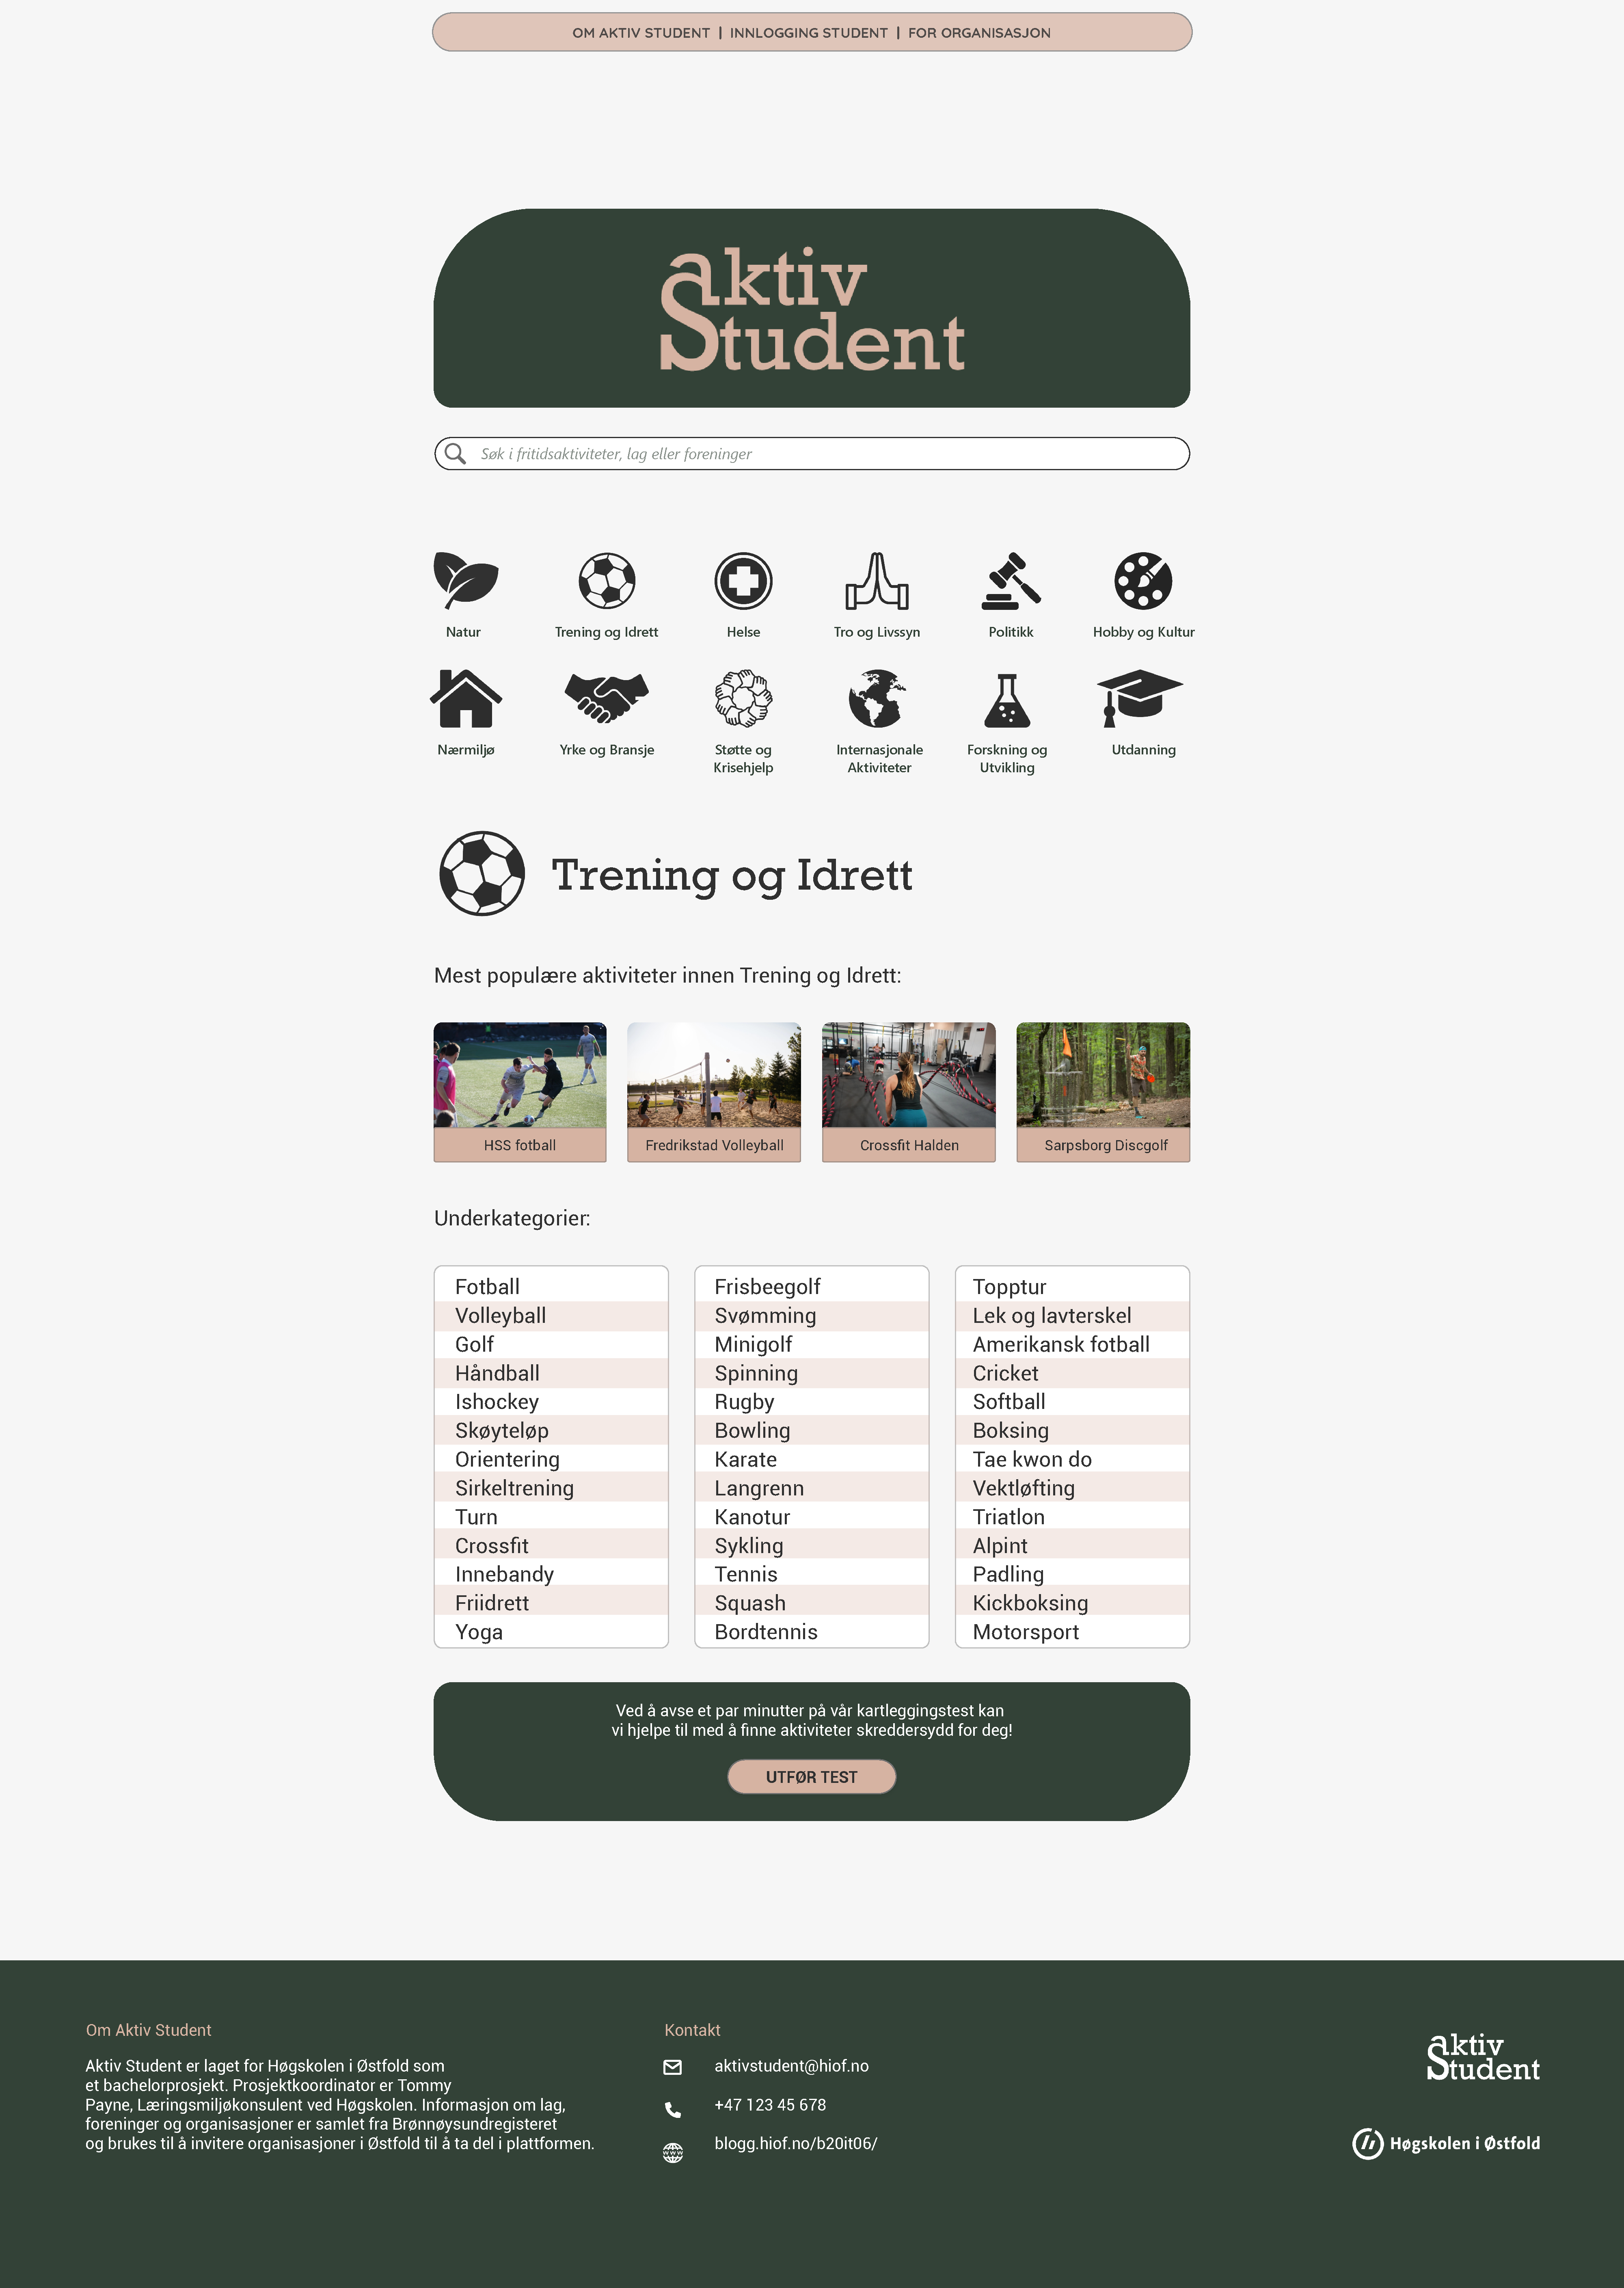
\includegraphics[width=.9\textwidth]{Illustrasjoner/Skisser-pdf/3.0/3-2-forside-trykket-kategori.pdf}
\caption{Adobe XD-skisse av plattformens forside etter bruker har trykket på kategori-ikonet for {\em Trening og Idrett}}
\label{vedlegg:3-2-forside-utbrett}
\end{figure}

\section{Søkeresultater}

\begin{figure}[H]
\centering
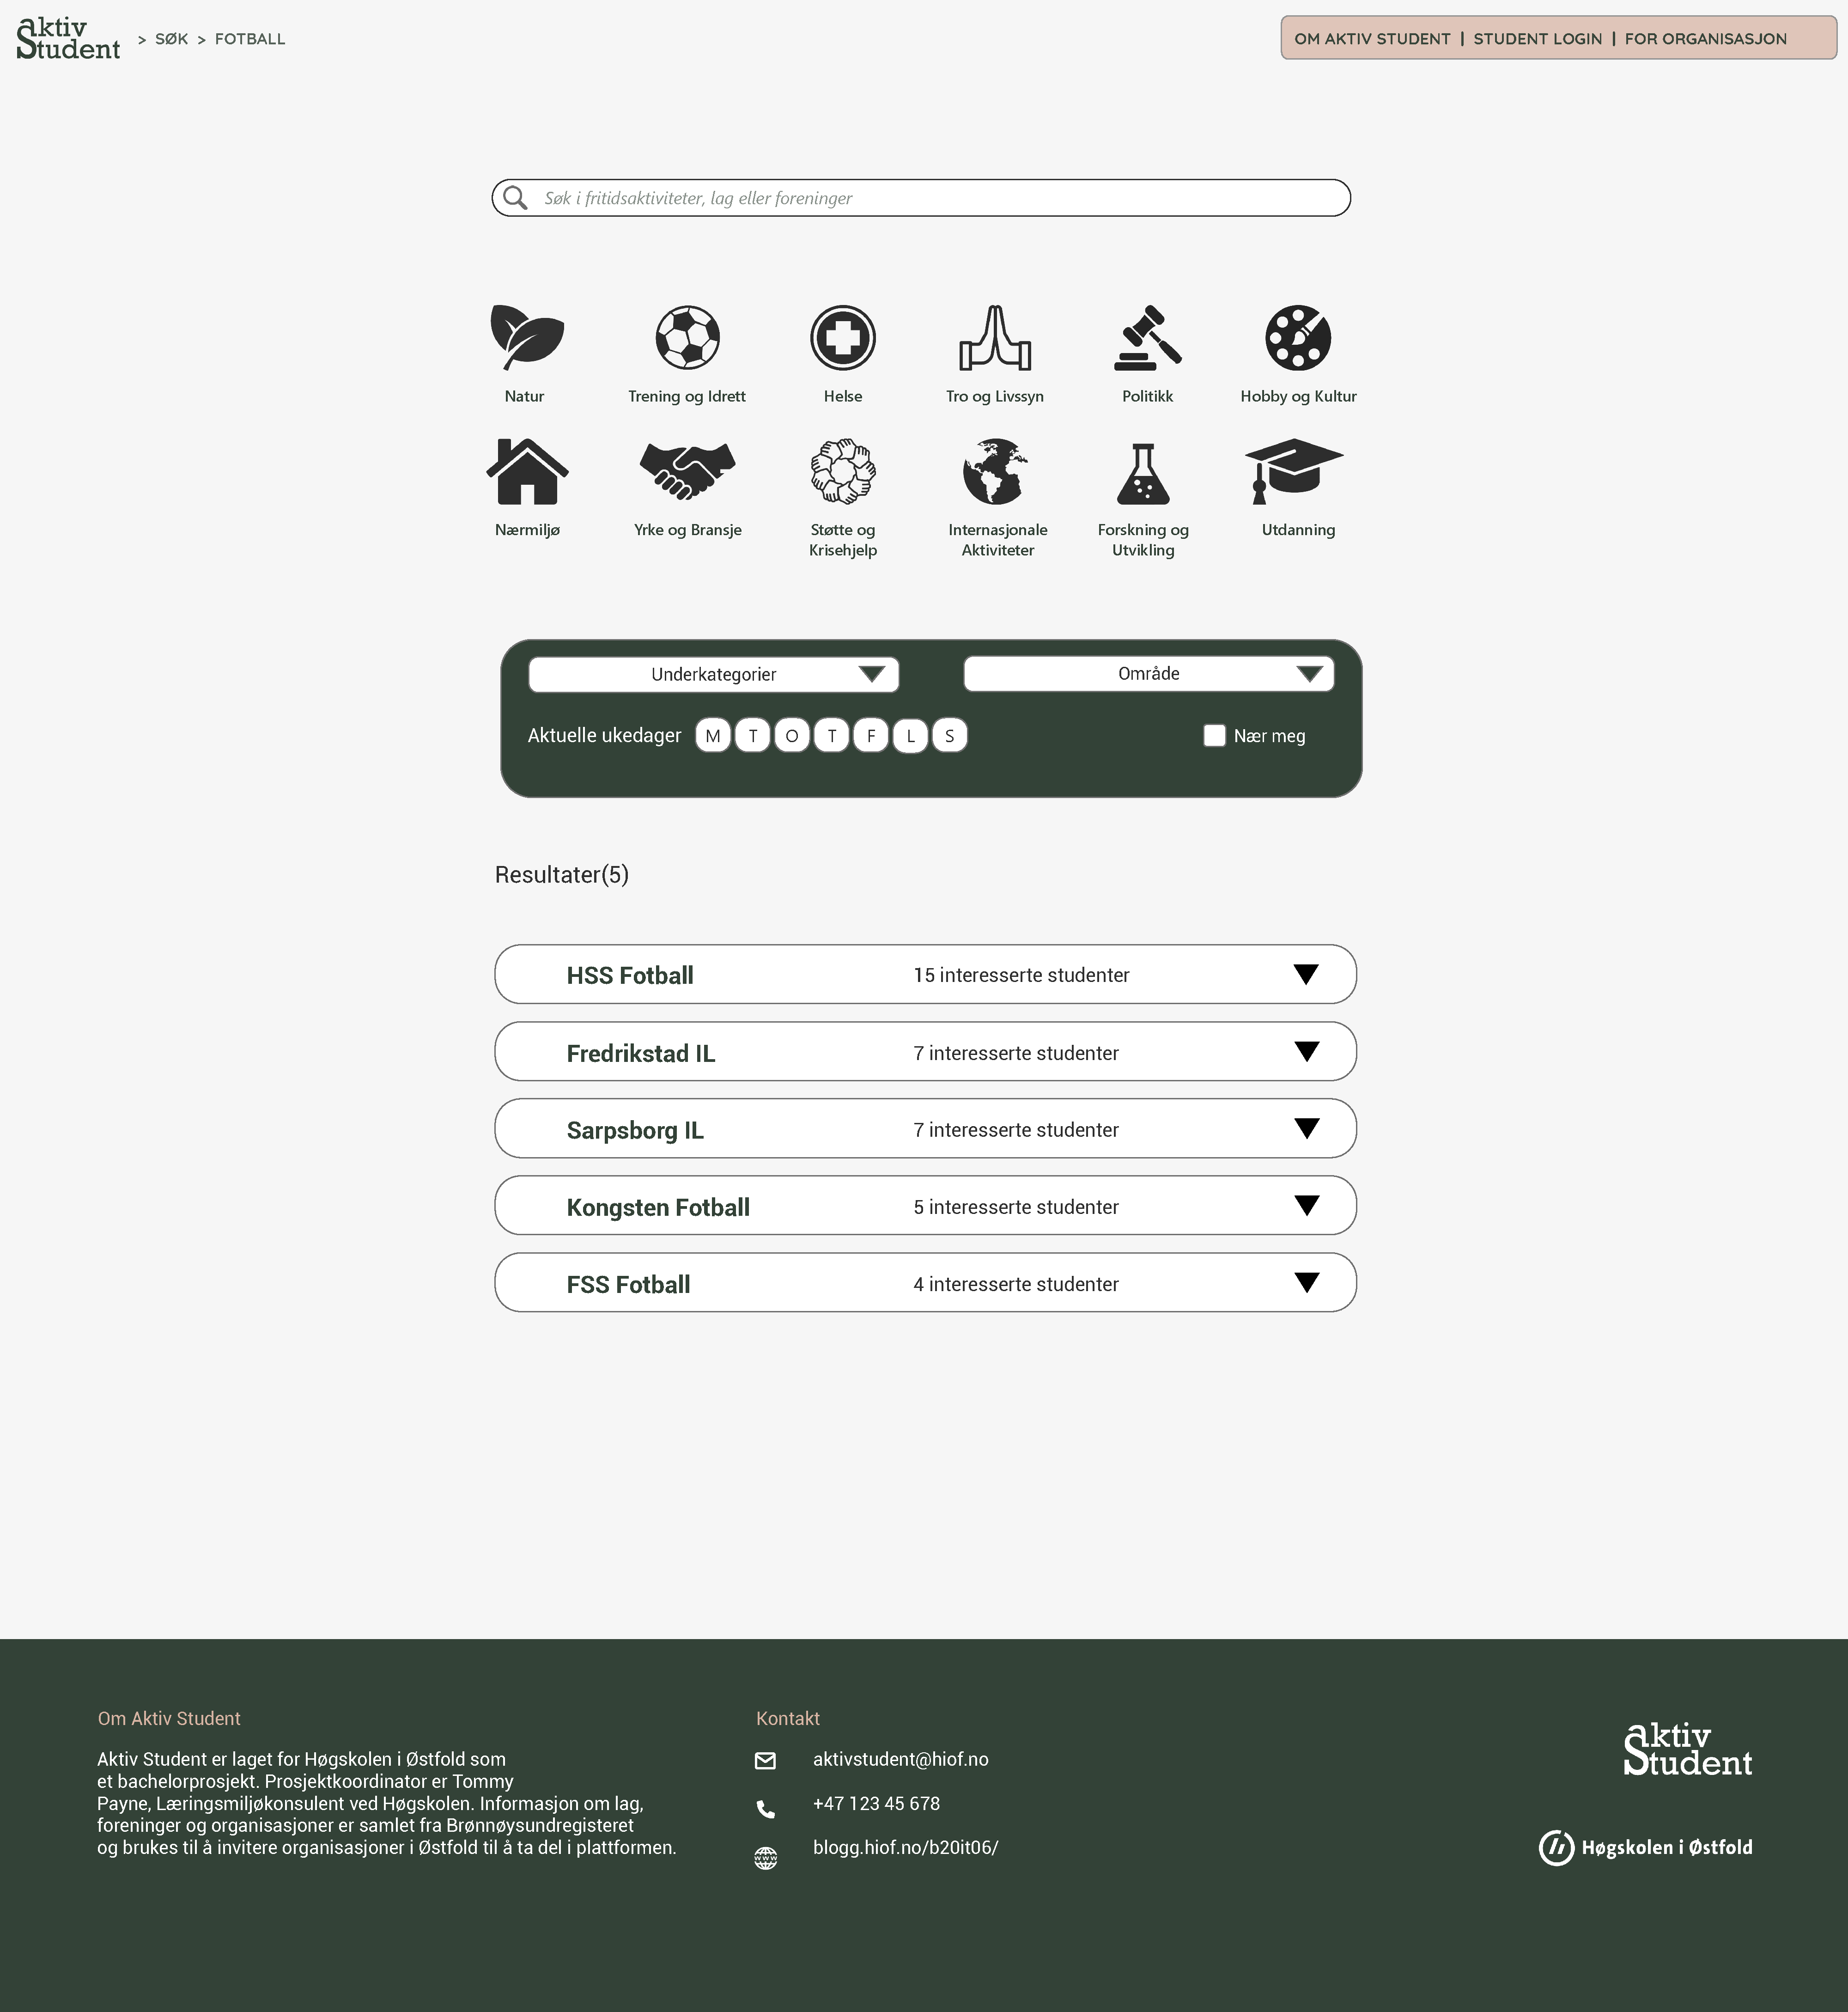
\includegraphics[width=\textwidth]{Illustrasjoner/Skisser-pdf/3.0/3-3-resultater-fotball.pdf}
\caption{Adobe XD-skisse av søkeresultatene etter bruker har trykket på underkategorien {\em Fotball}}
\label{vedlegg:3-3-resultater-filtrering}
\end{figure}

\section{Organisasjonsside}

\begin{figure}[H]
\centering
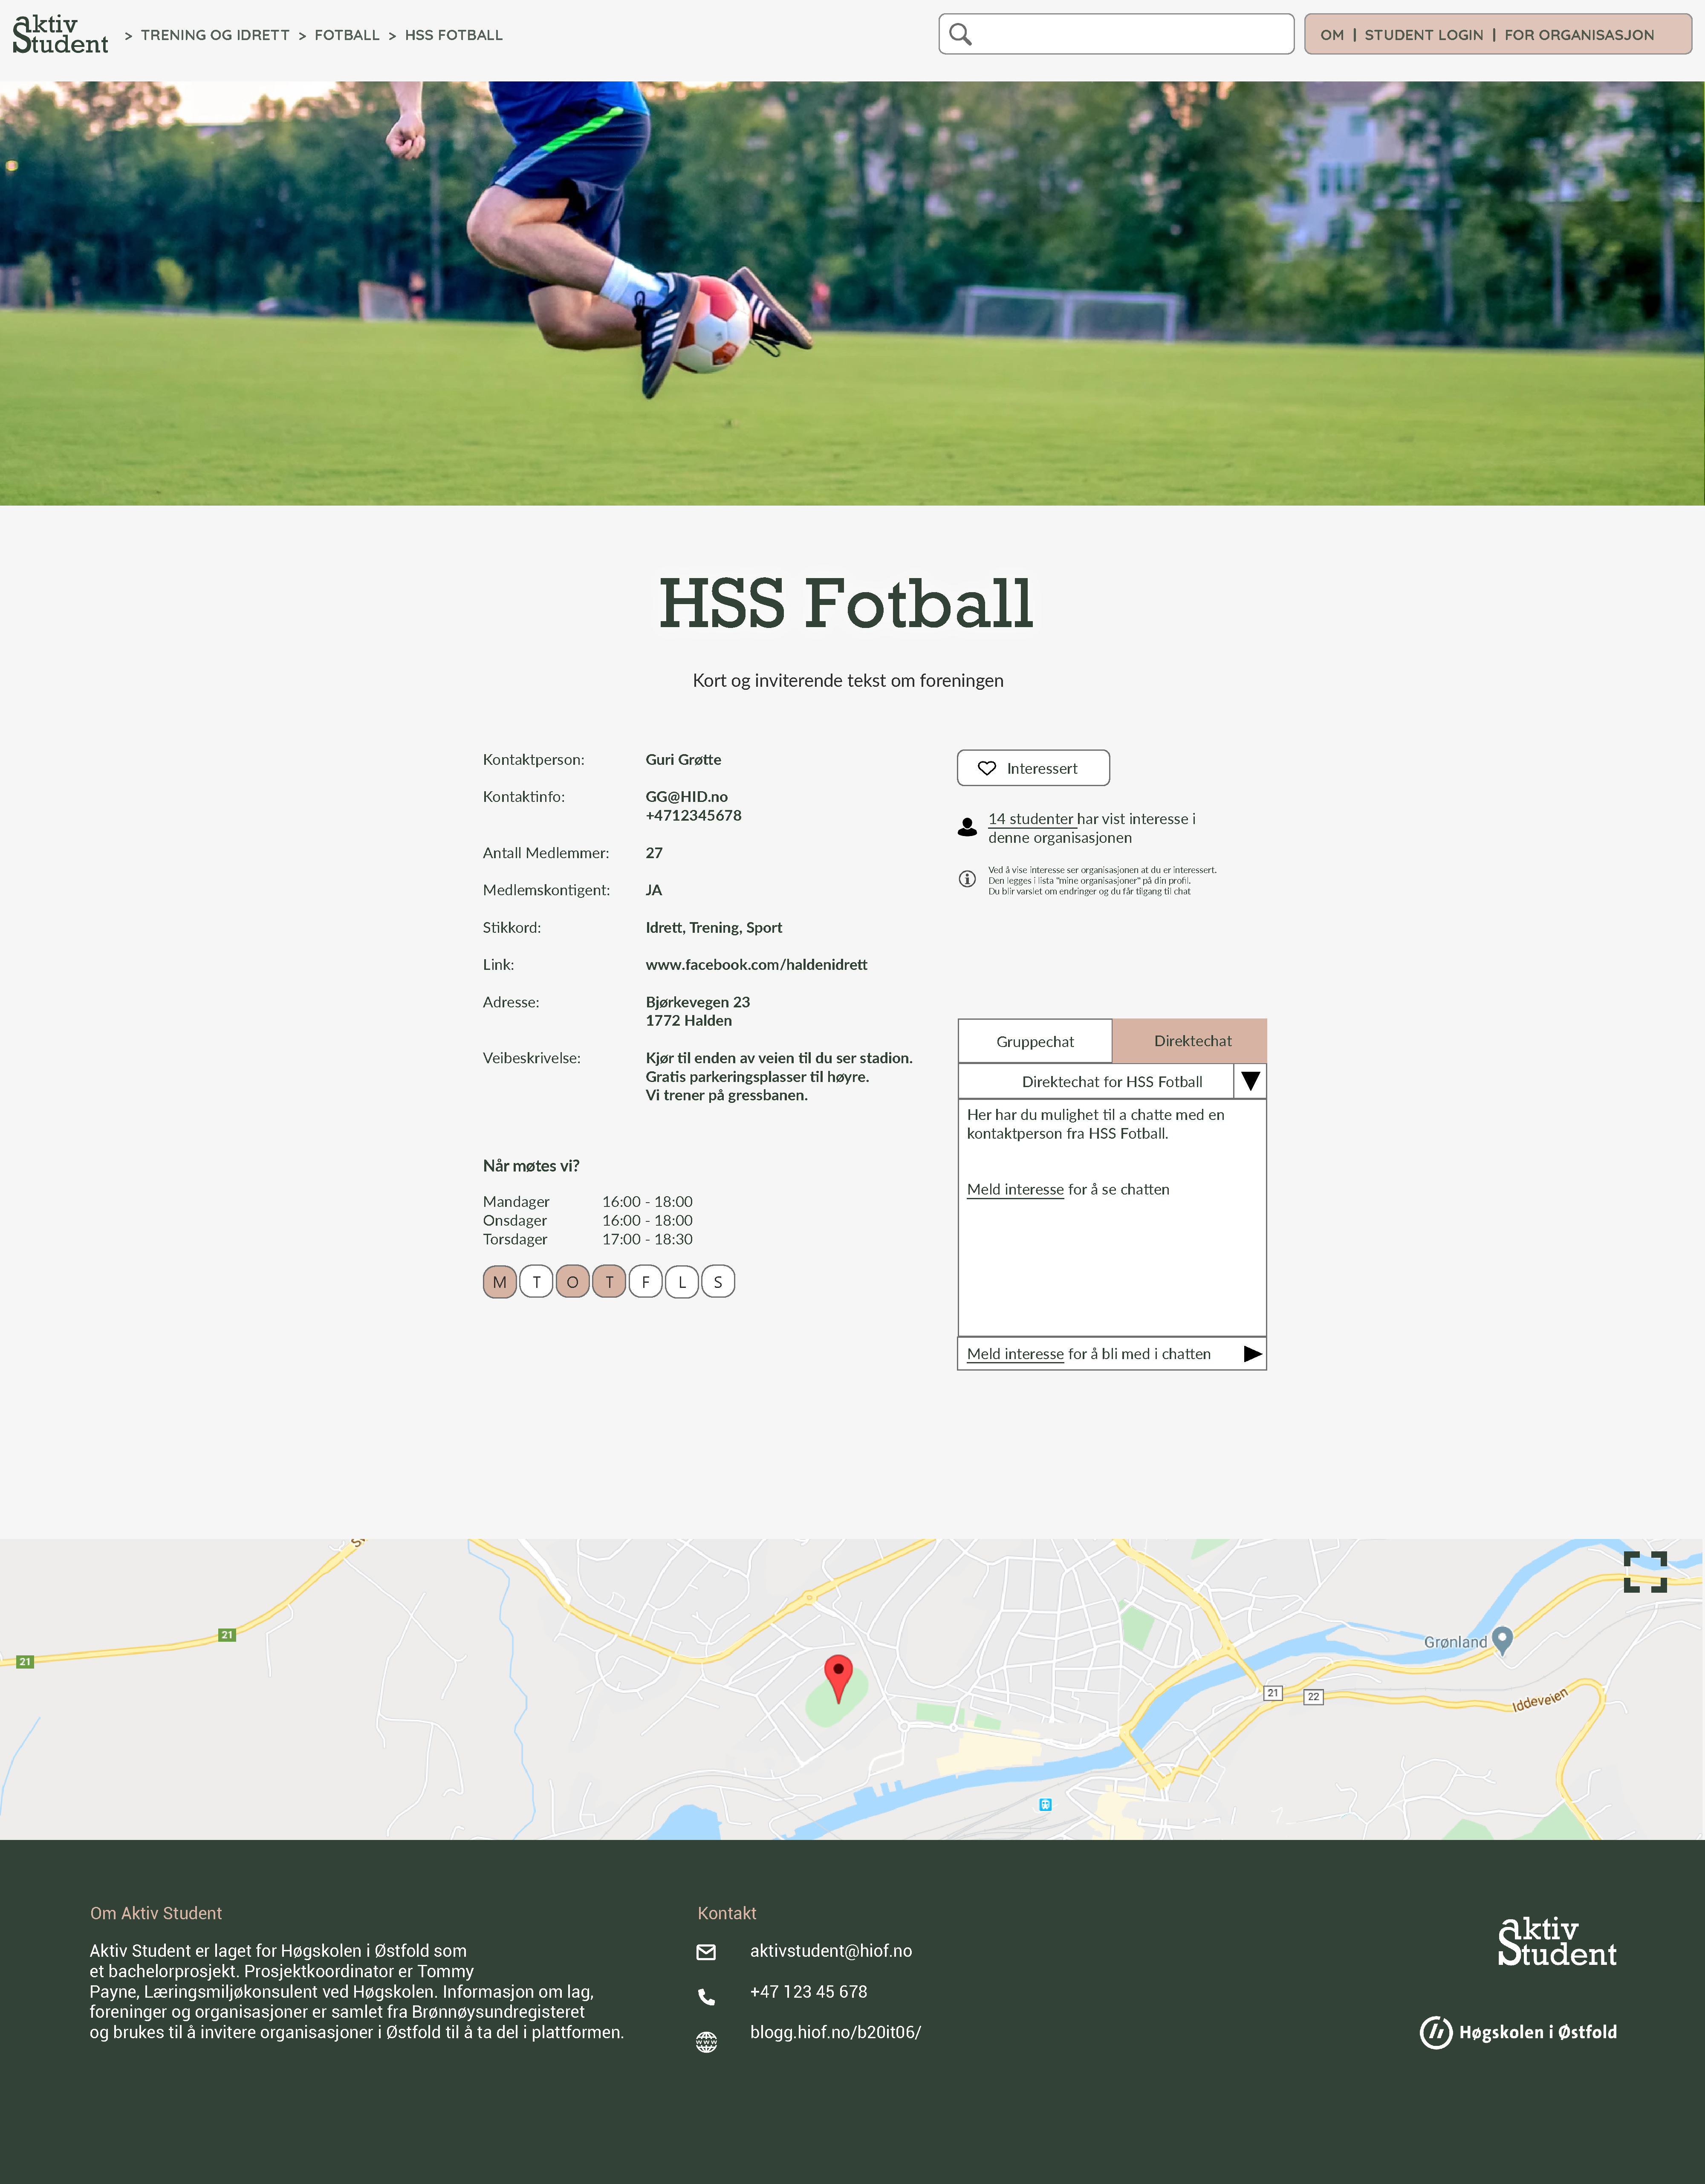
\includegraphics[width=\textwidth]{Illustrasjoner/Skisser-pdf/3.0/3-4-organisasjonsside.pdf}
\caption{Adobe XD-skisse av siden til eksempelorganisasjonen {\em HSS Fotball}}
\label{vedlegg:3-4-org-side}
\end{figure}

\section{Andre interesserte studenter}

\begin{figure}[H]
\centering
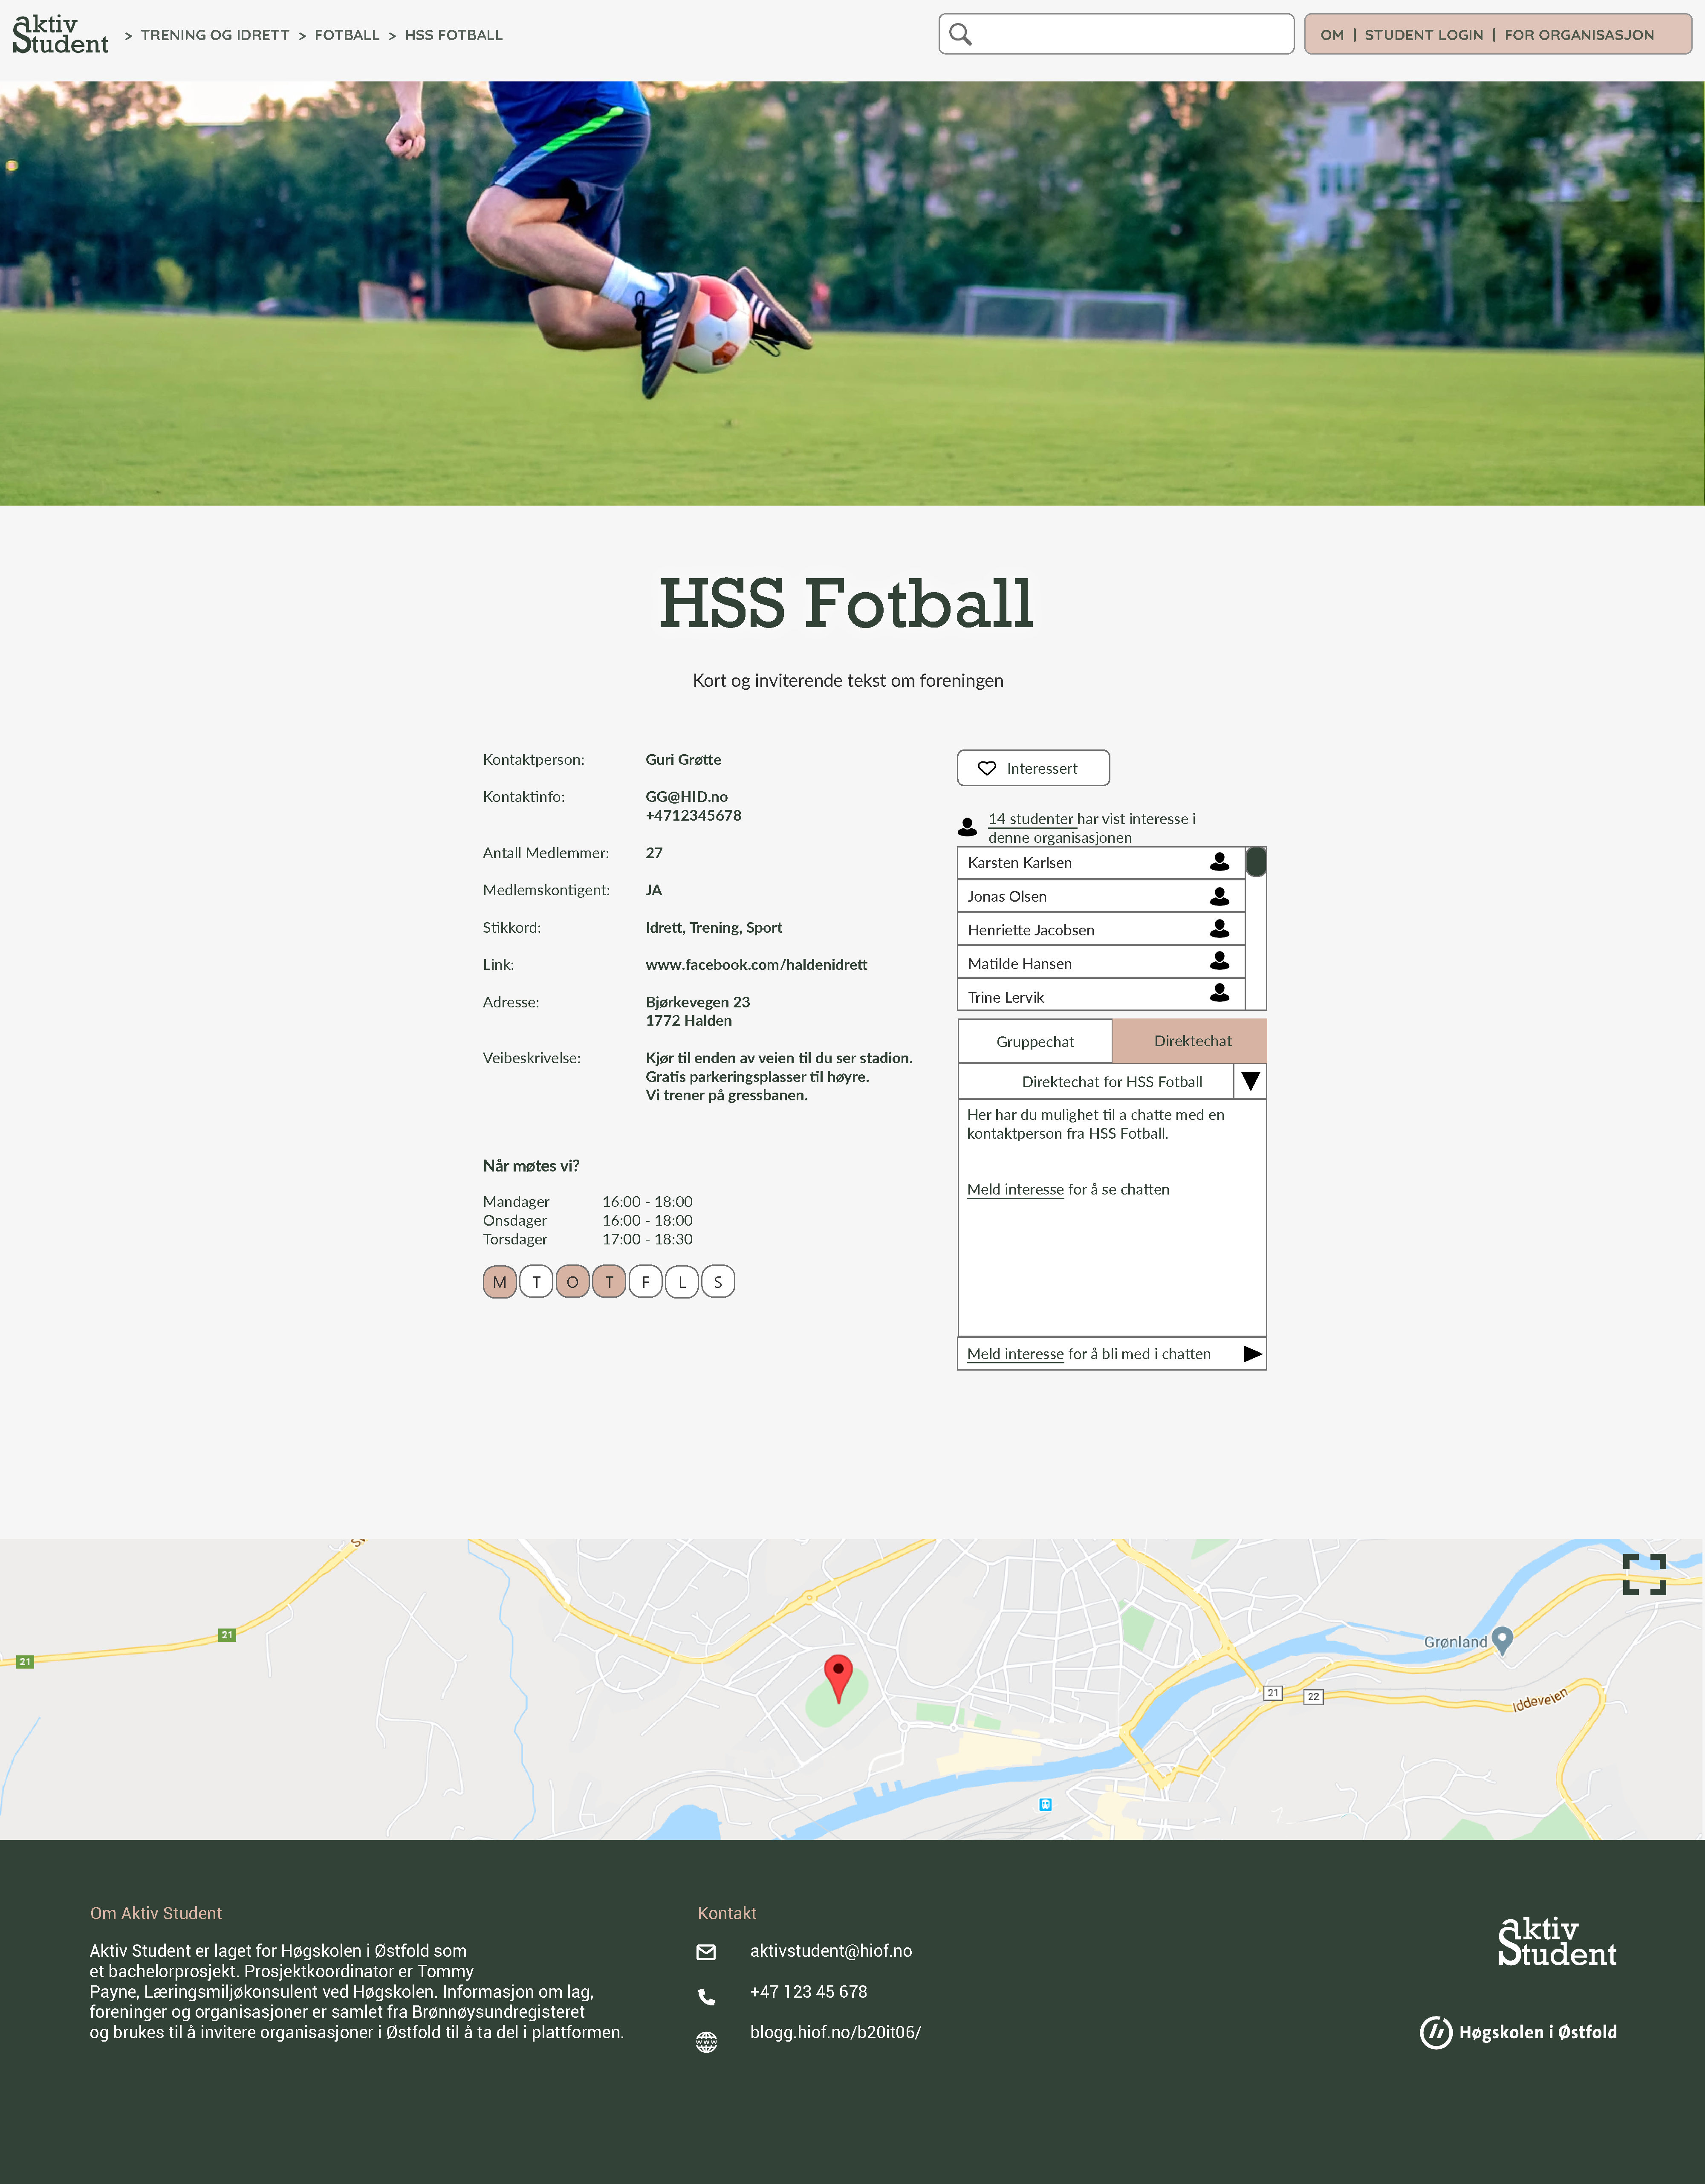
\includegraphics[width=\textwidth]{Illustrasjoner/Skisser-pdf/3.0/3-5-interesserte-organisasjon.pdf}
\caption{Adobe XD-skisse av siden til eksempelorganisasjonen {\em HSS Fotball} etter bruker har trykket på linken i teksten {\em 14 studenter har vist interesse for denne organisasjonen}}
\label{vedlegg:3-5-andre-interesserte-org}
\end{figure}

\section{Organisasjonsside etter bruker har trykket {\em interessert}}

\begin{figure}[H]
\centering
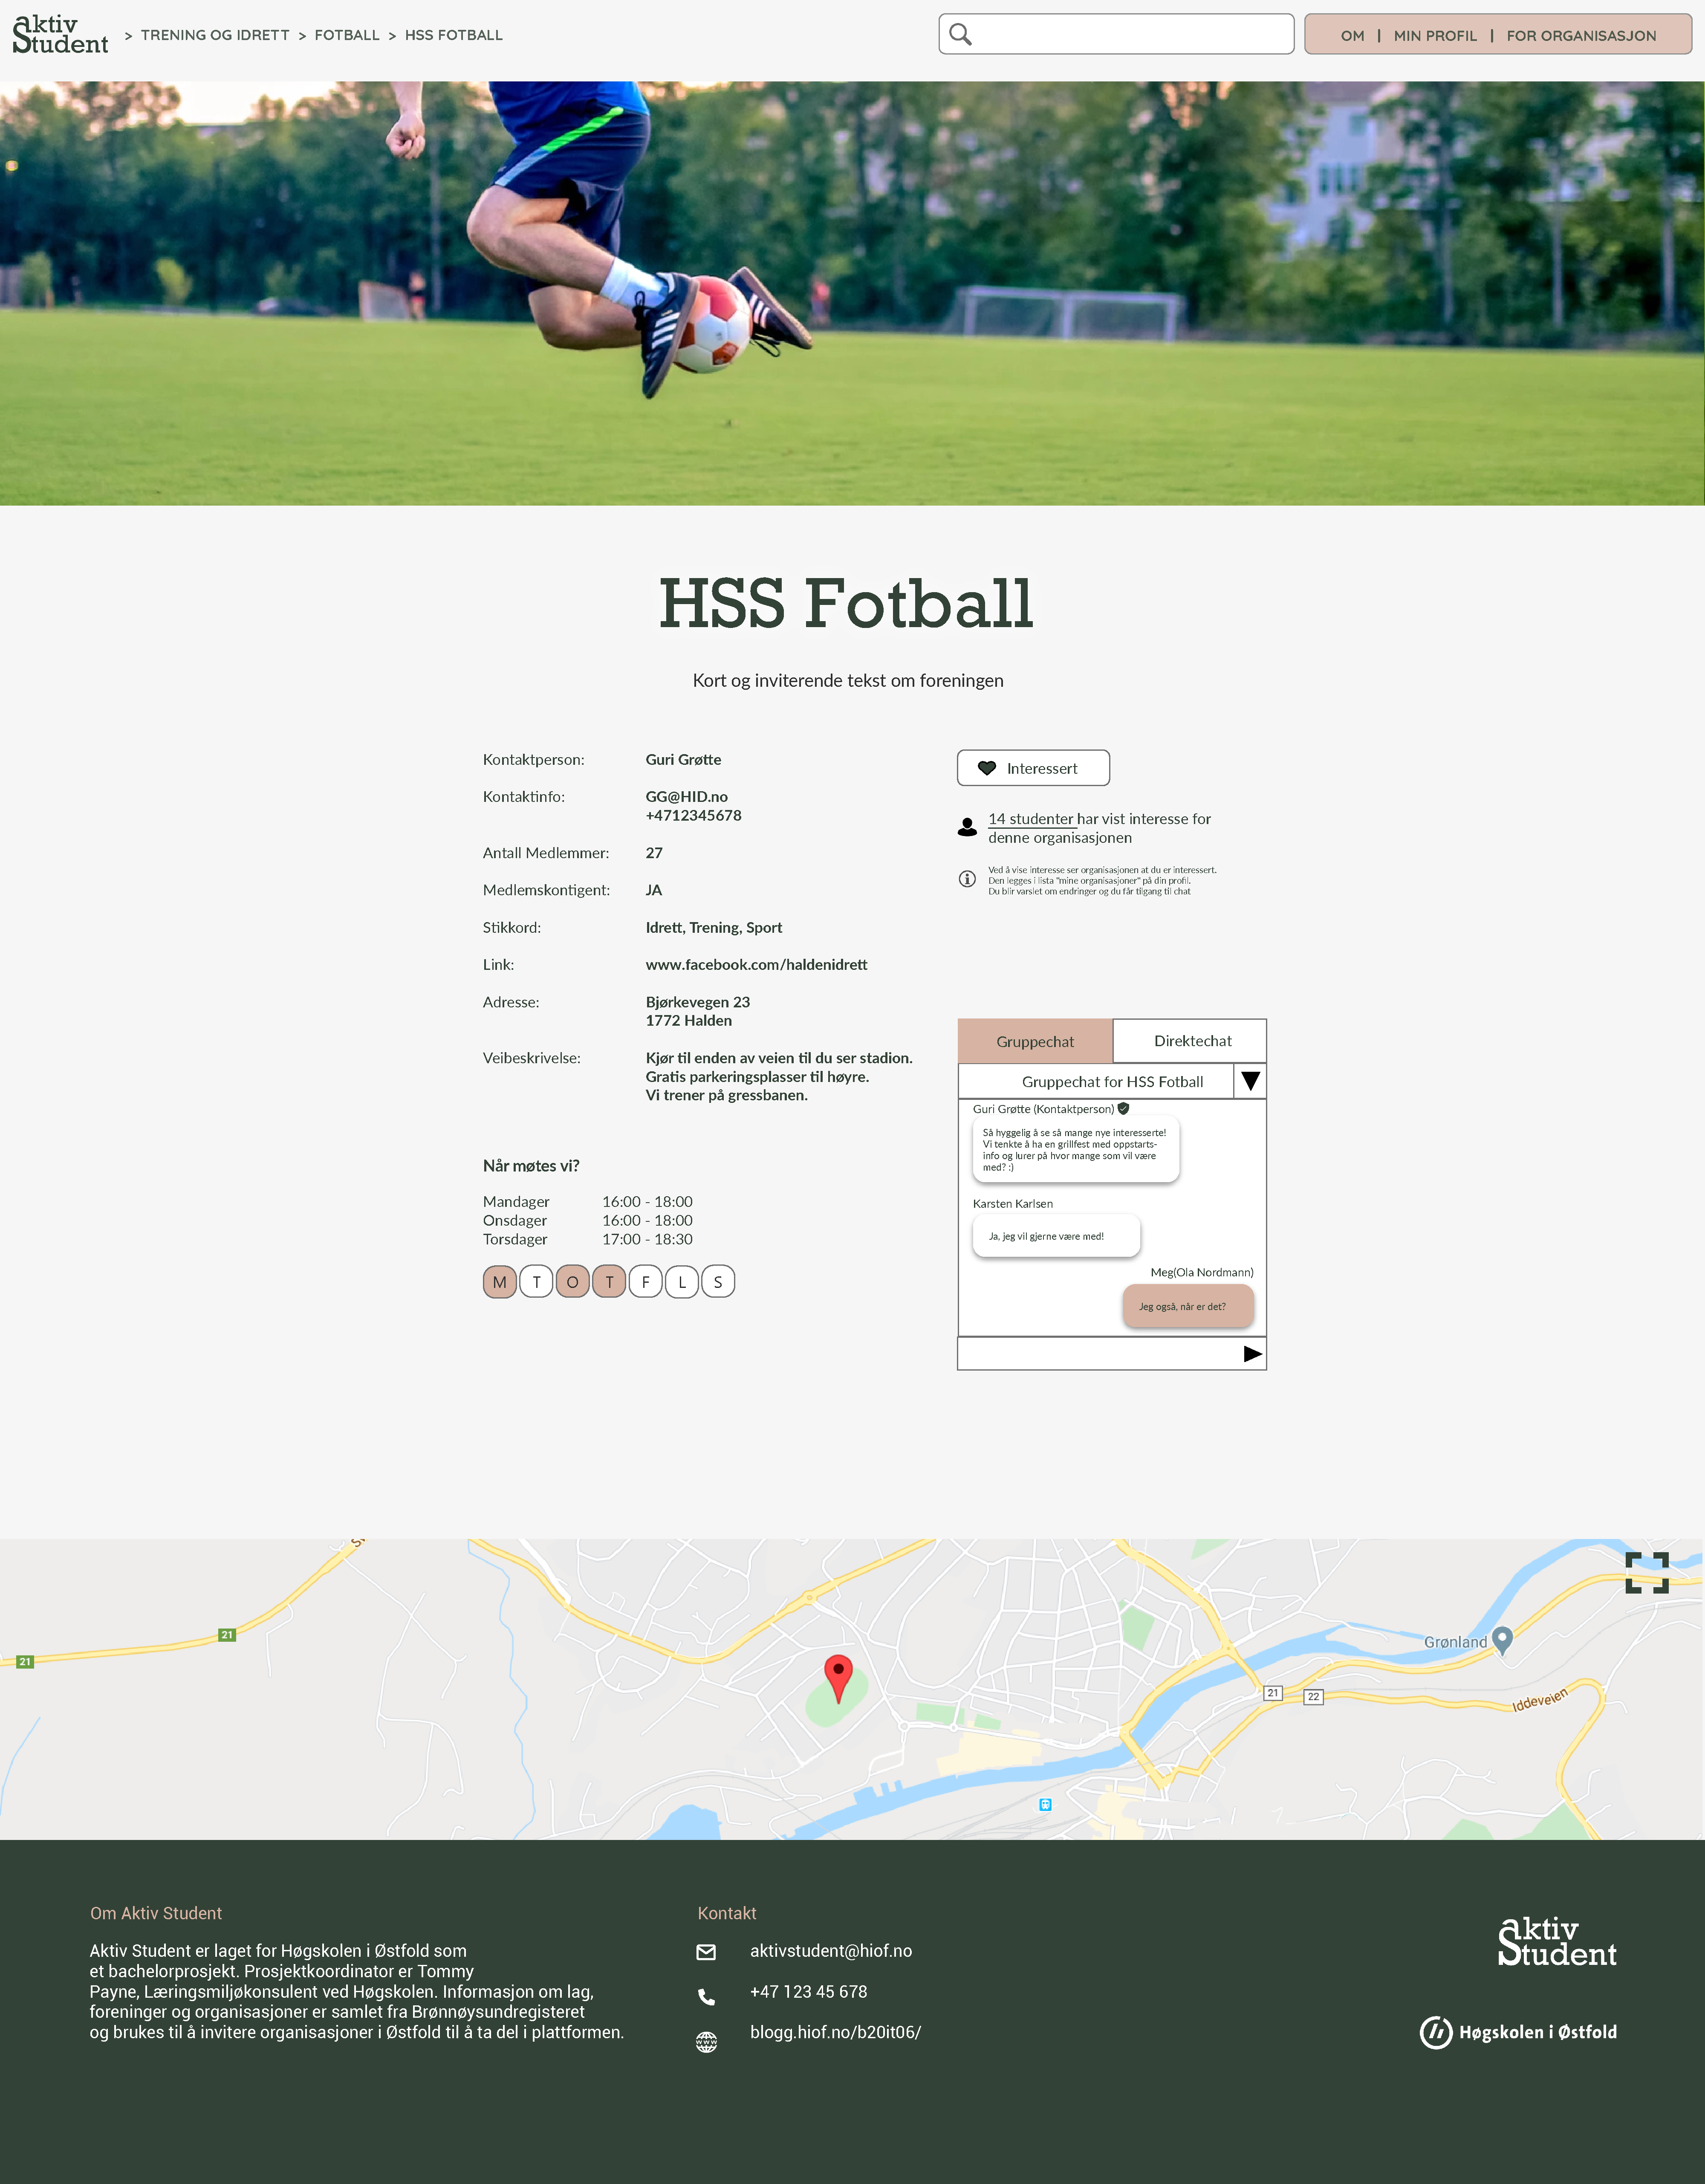
\includegraphics[width=\textwidth]{Illustrasjoner/Skisser-pdf/3.0/3-6-organisasjonsside-trykket-interessert.pdf}
\caption{Adobe XD-skisse av siden til eksempelorganisasjonen HSS Fotball etter bruker har trykket på {\em interessert}-knappen og får tilgang til chattefunksjonen}
\label{vedlegg:3-6-org-trykket-interessert}
\end{figure}

\section{Annen brukers profil}

\begin{figure}[H]
\centering
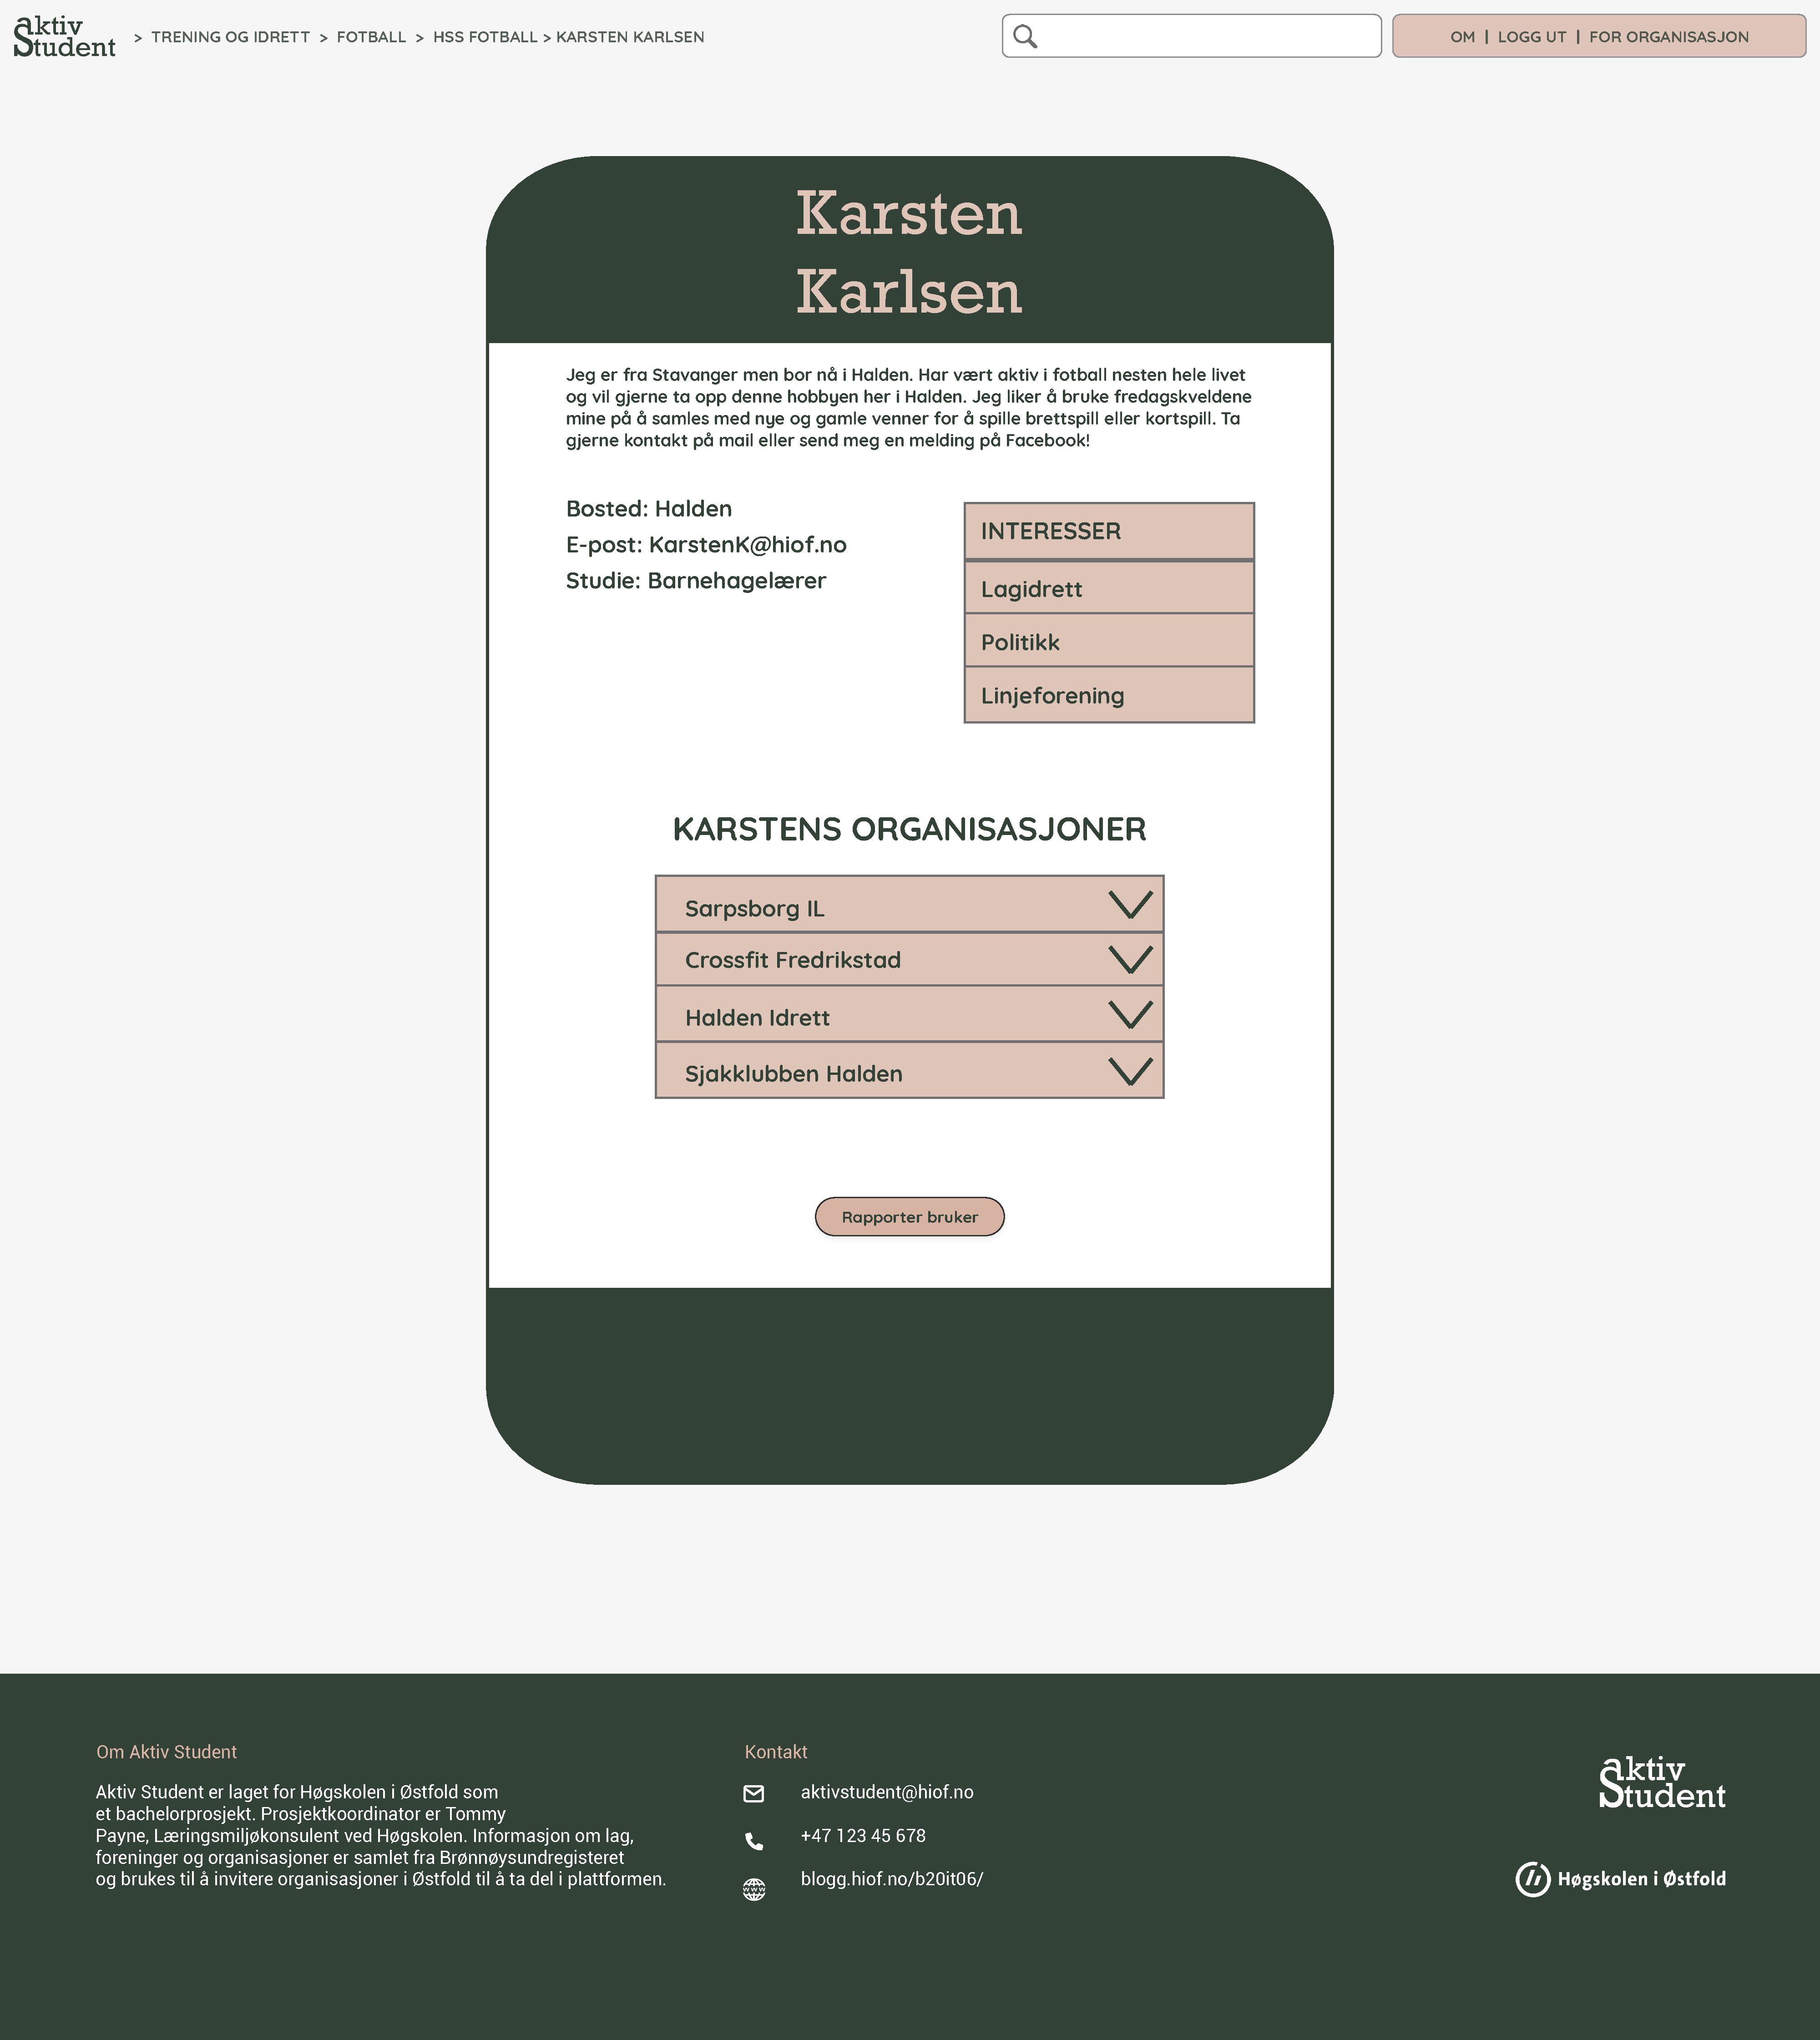
\includegraphics[width=\textwidth]{Illustrasjoner/Skisser-pdf/3.0/3-7-annen-brukers-profil.pdf}
\caption{Adobe XD-skisse av profilen til en annen bruker}
\label{vedlegg:3-7-annen-bruker}
\end{figure}

\section{Oppretting av brukerprofil}

\begin{figure}[H]
\centering
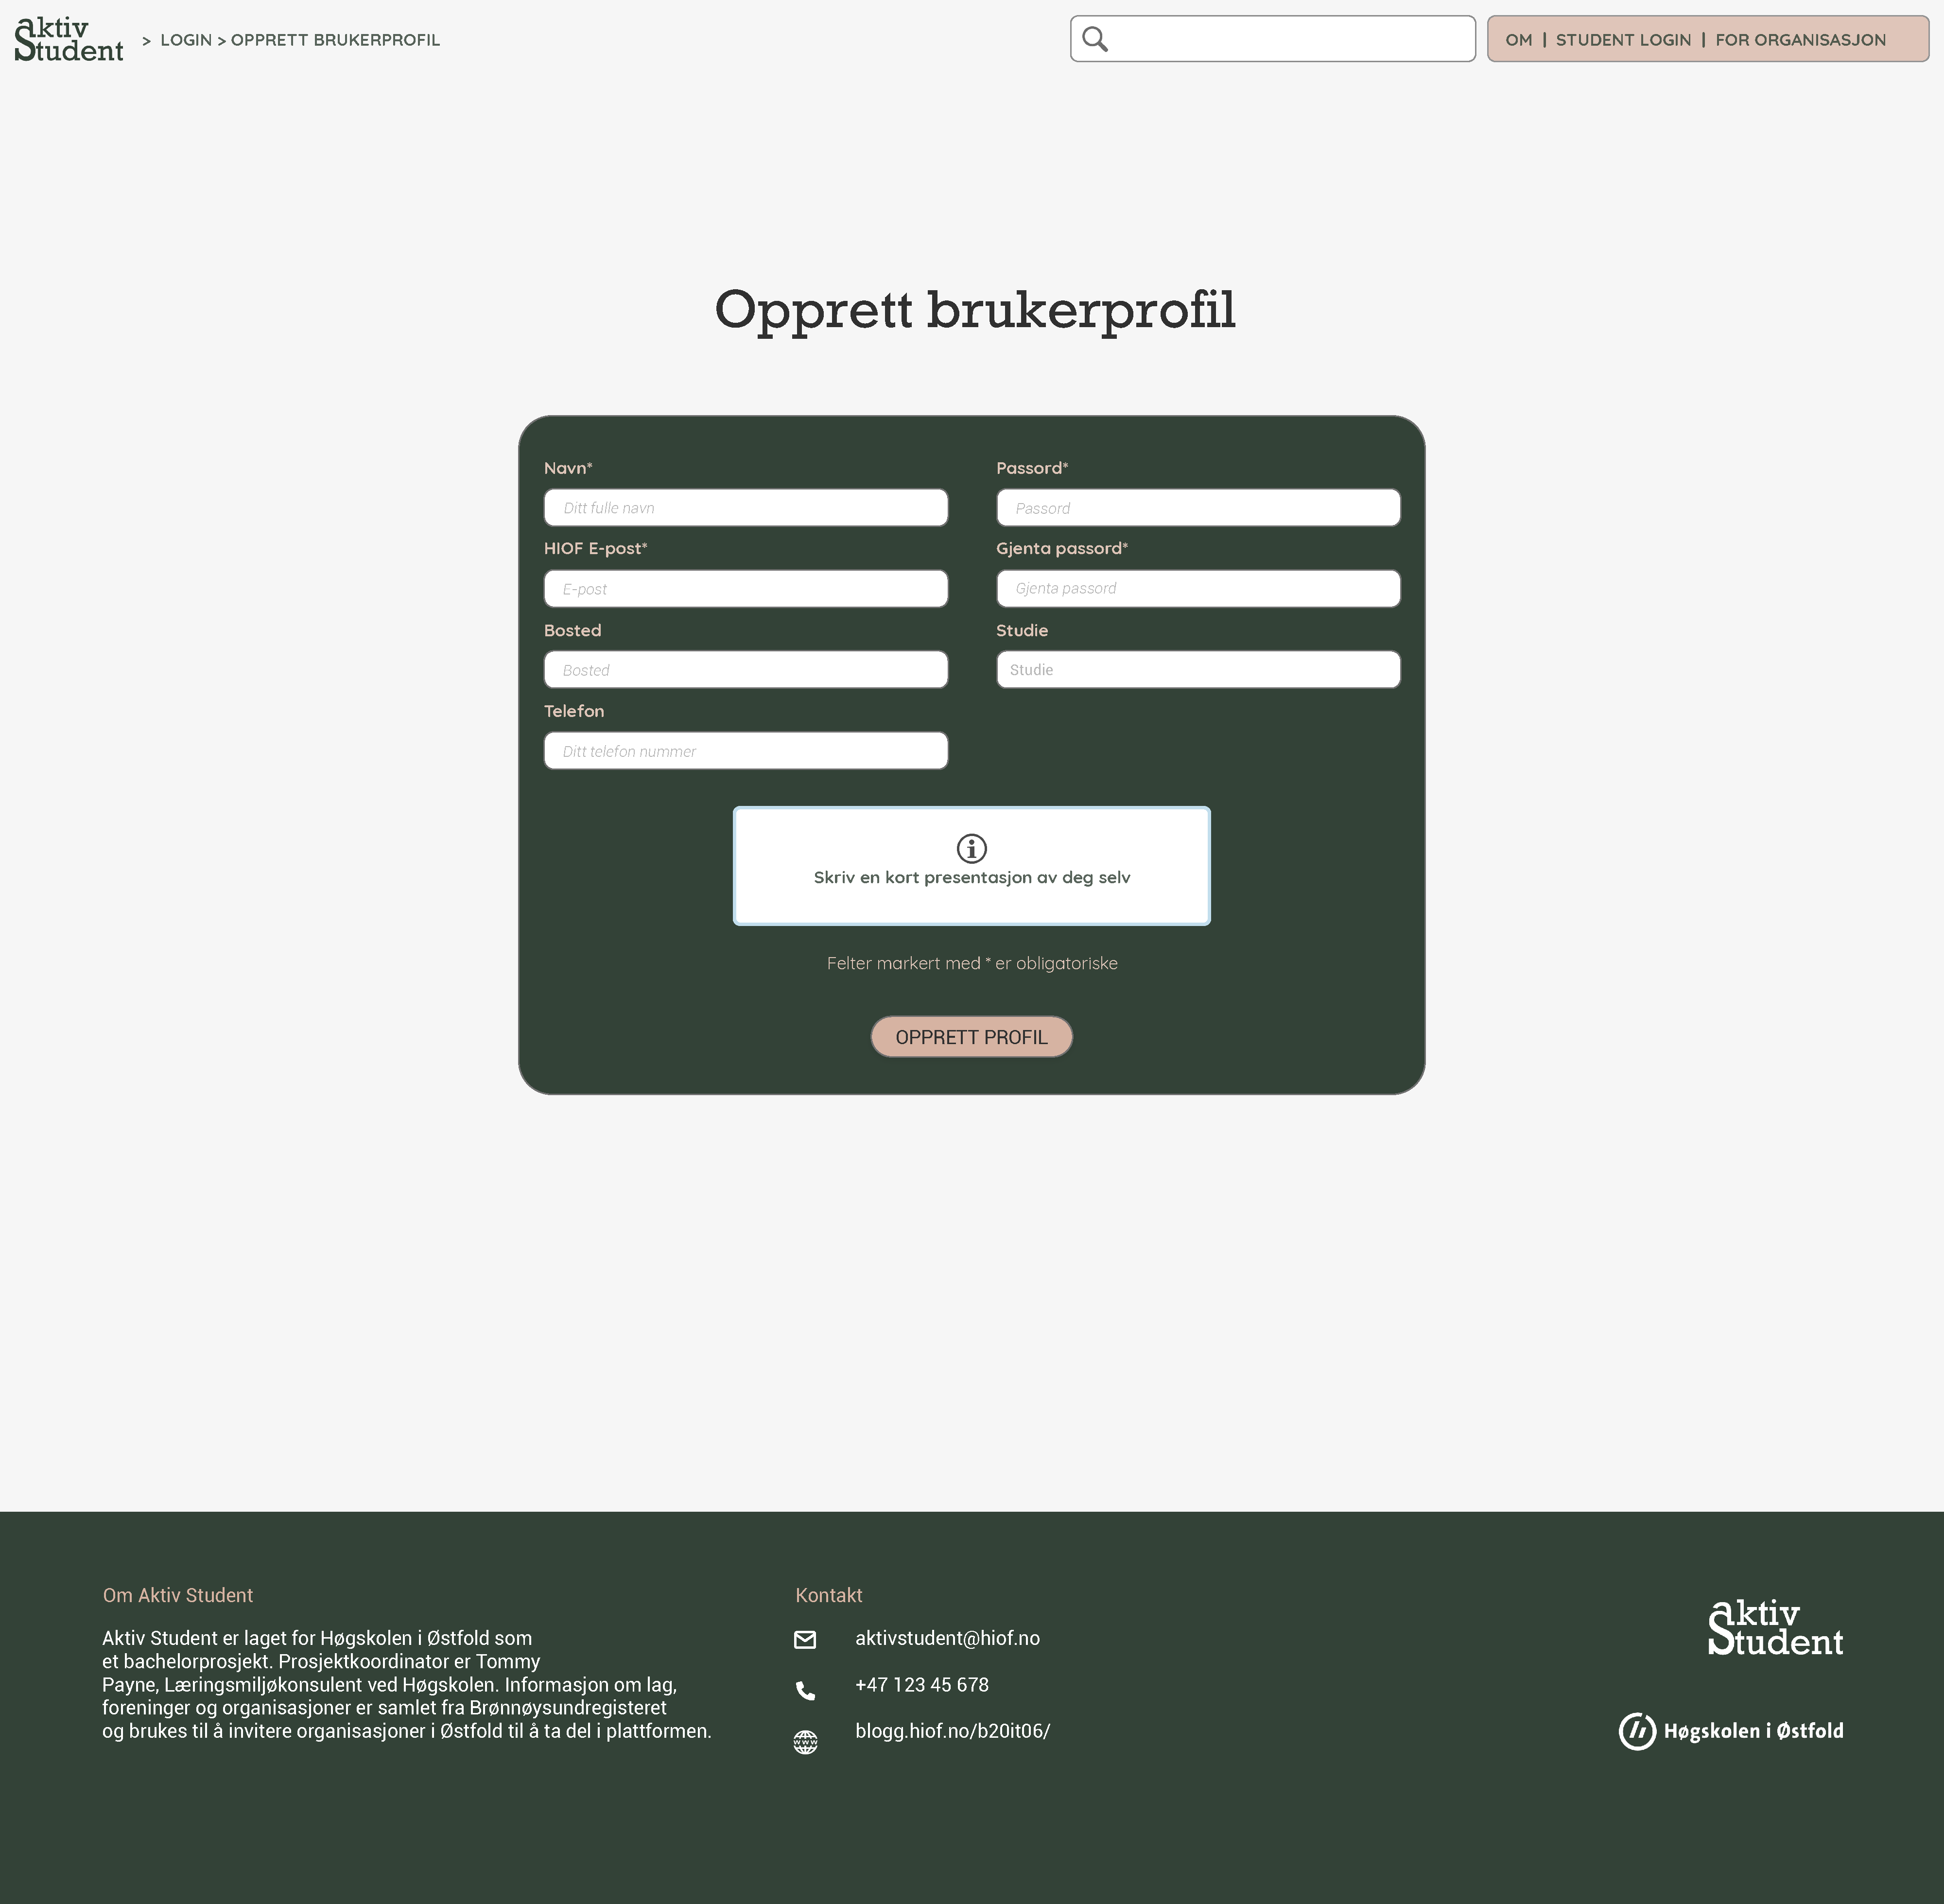
\includegraphics[width=\textwidth]{Illustrasjoner/Skisser-pdf/3.0/3-8-opprett-brukerprofil.pdf}
\caption{Adobe XD-skisse av siden for å opprette ny brukerprofil}
\label{vedlegg:3-8-opprett-brukerprofil}
\end{figure}

\section{Innlogging for bruker}

\begin{figure}[H]
\centering
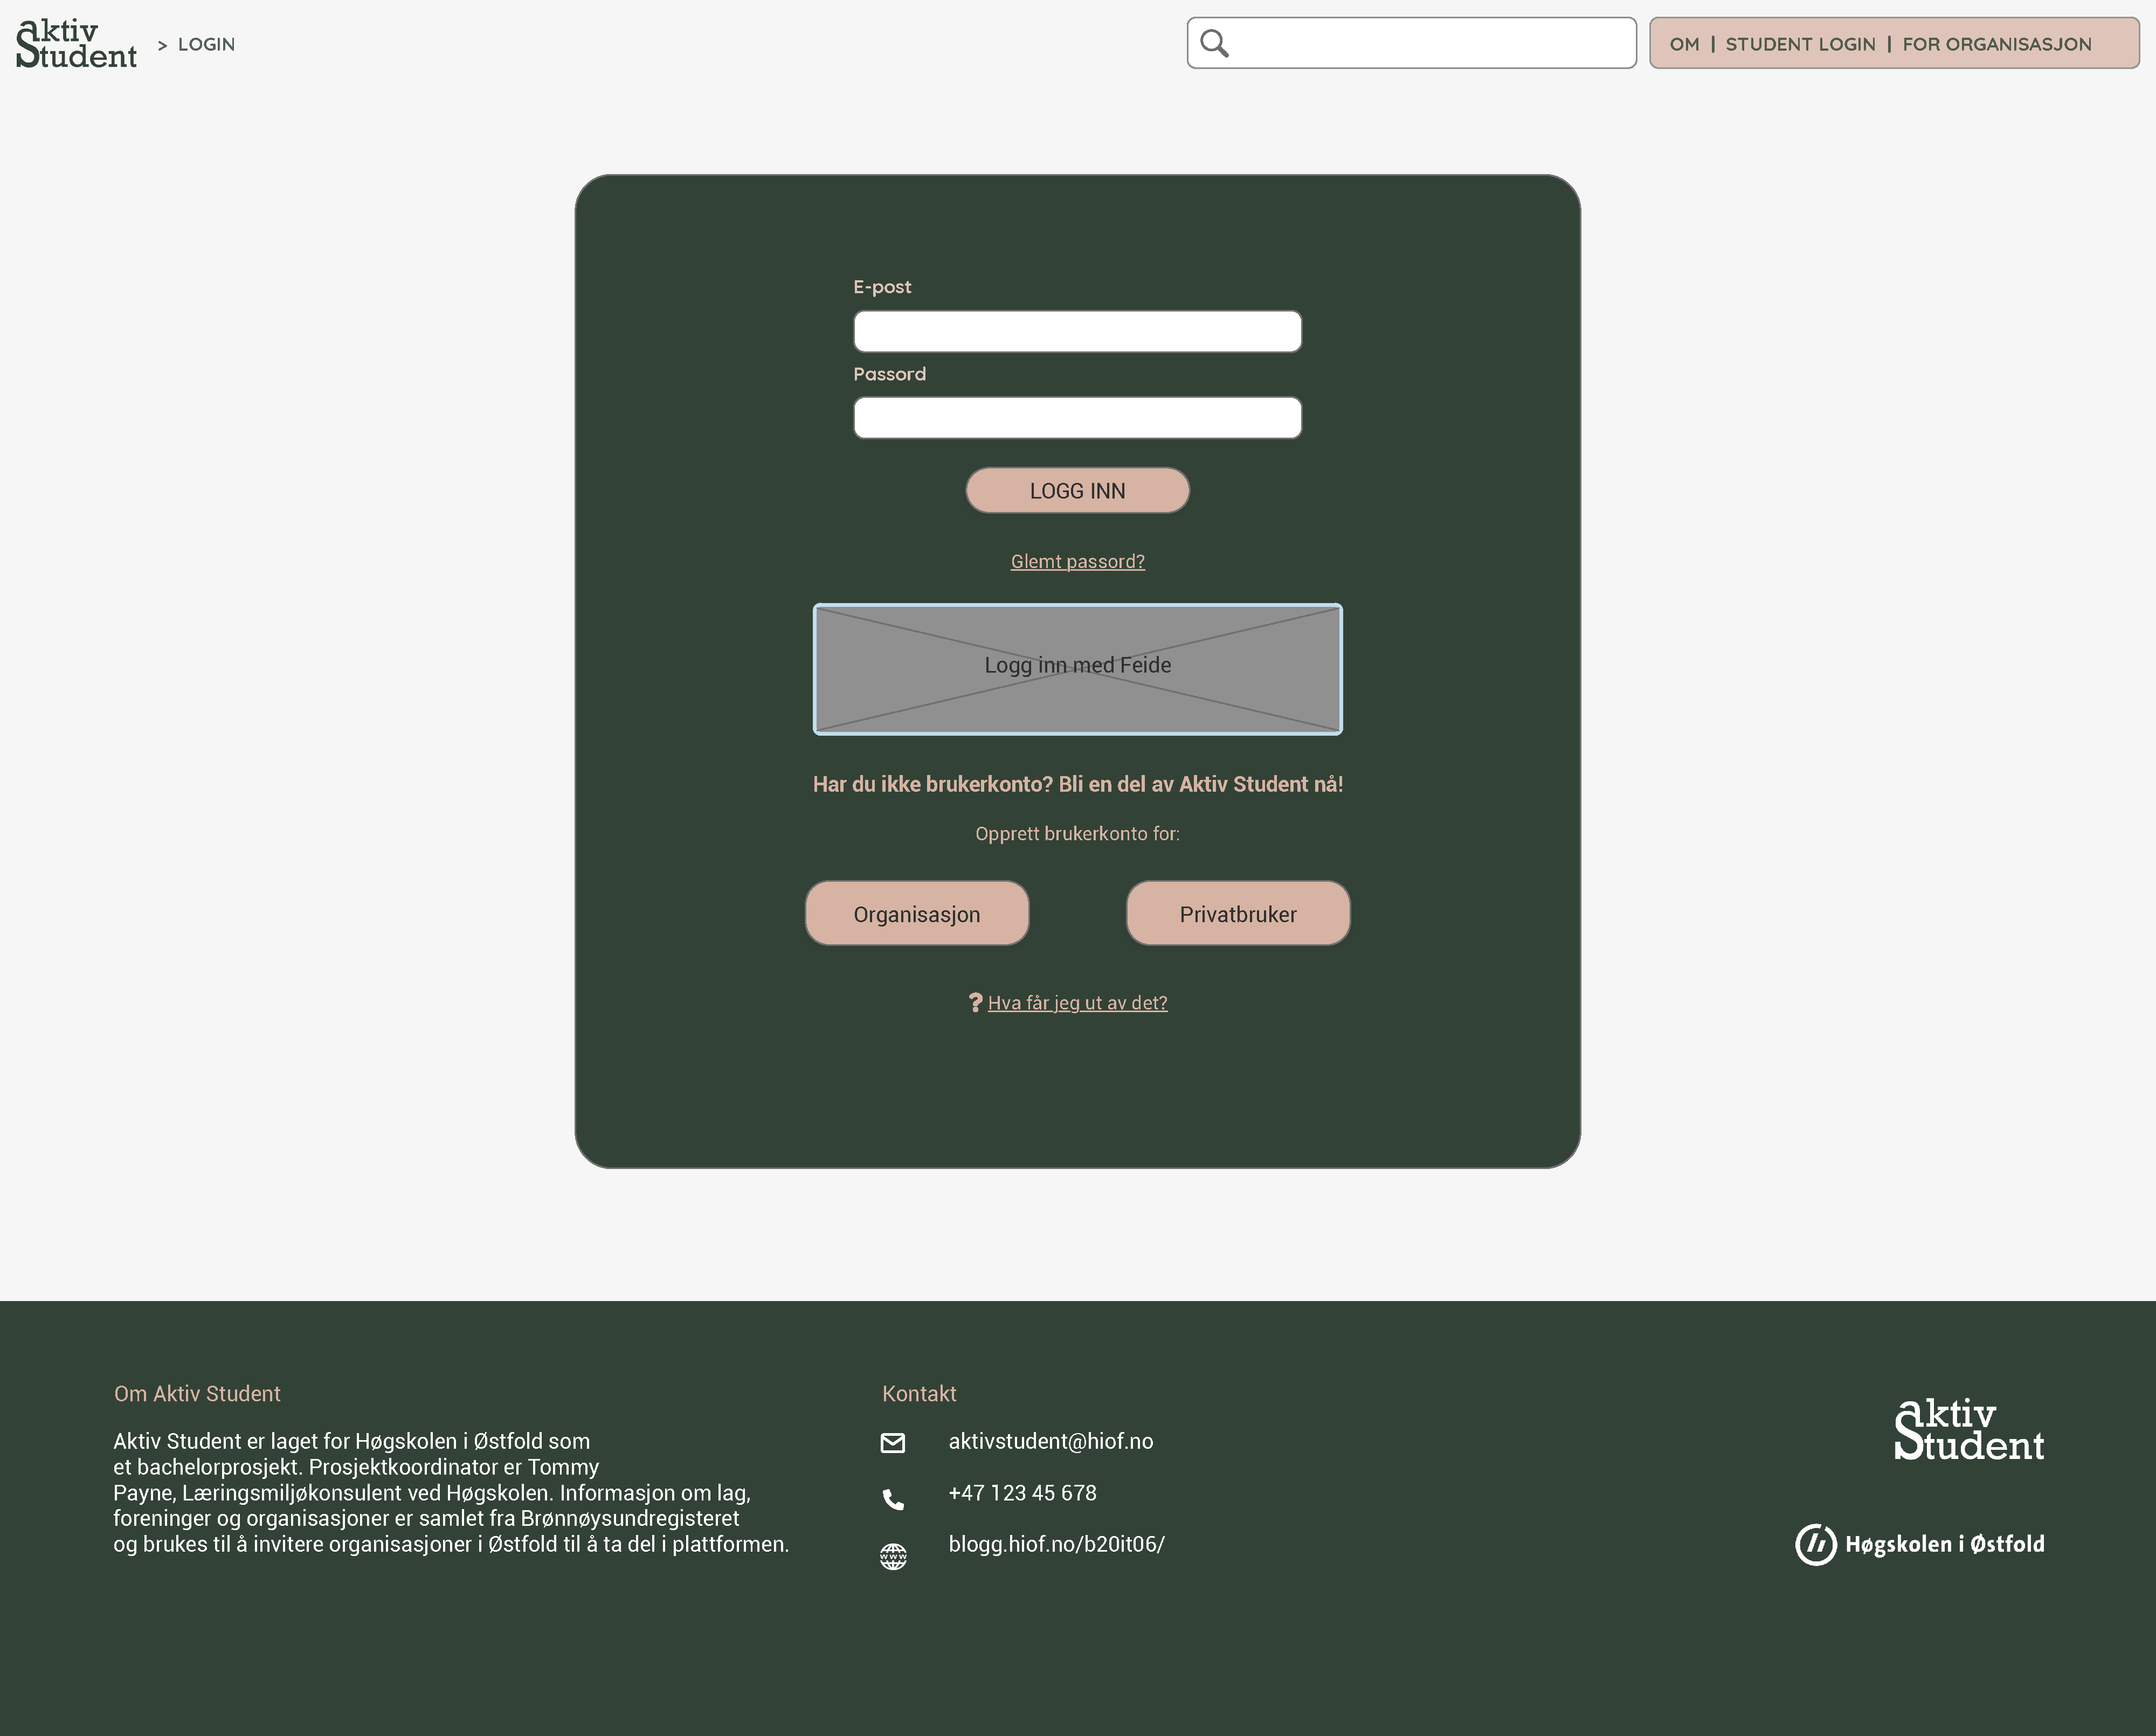
\includegraphics[width=\textwidth]{Illustrasjoner/Skisser-pdf/3.0/3-9-logg-inn.pdf}
\caption{Adobe XD-skisse av siden for å logge inn som privatbruker}
\label{vedlegg:3-9-innlogging-bruker}
\end{figure}

\section{Innlogget brukers profil}

\begin{figure}[H]
\centering
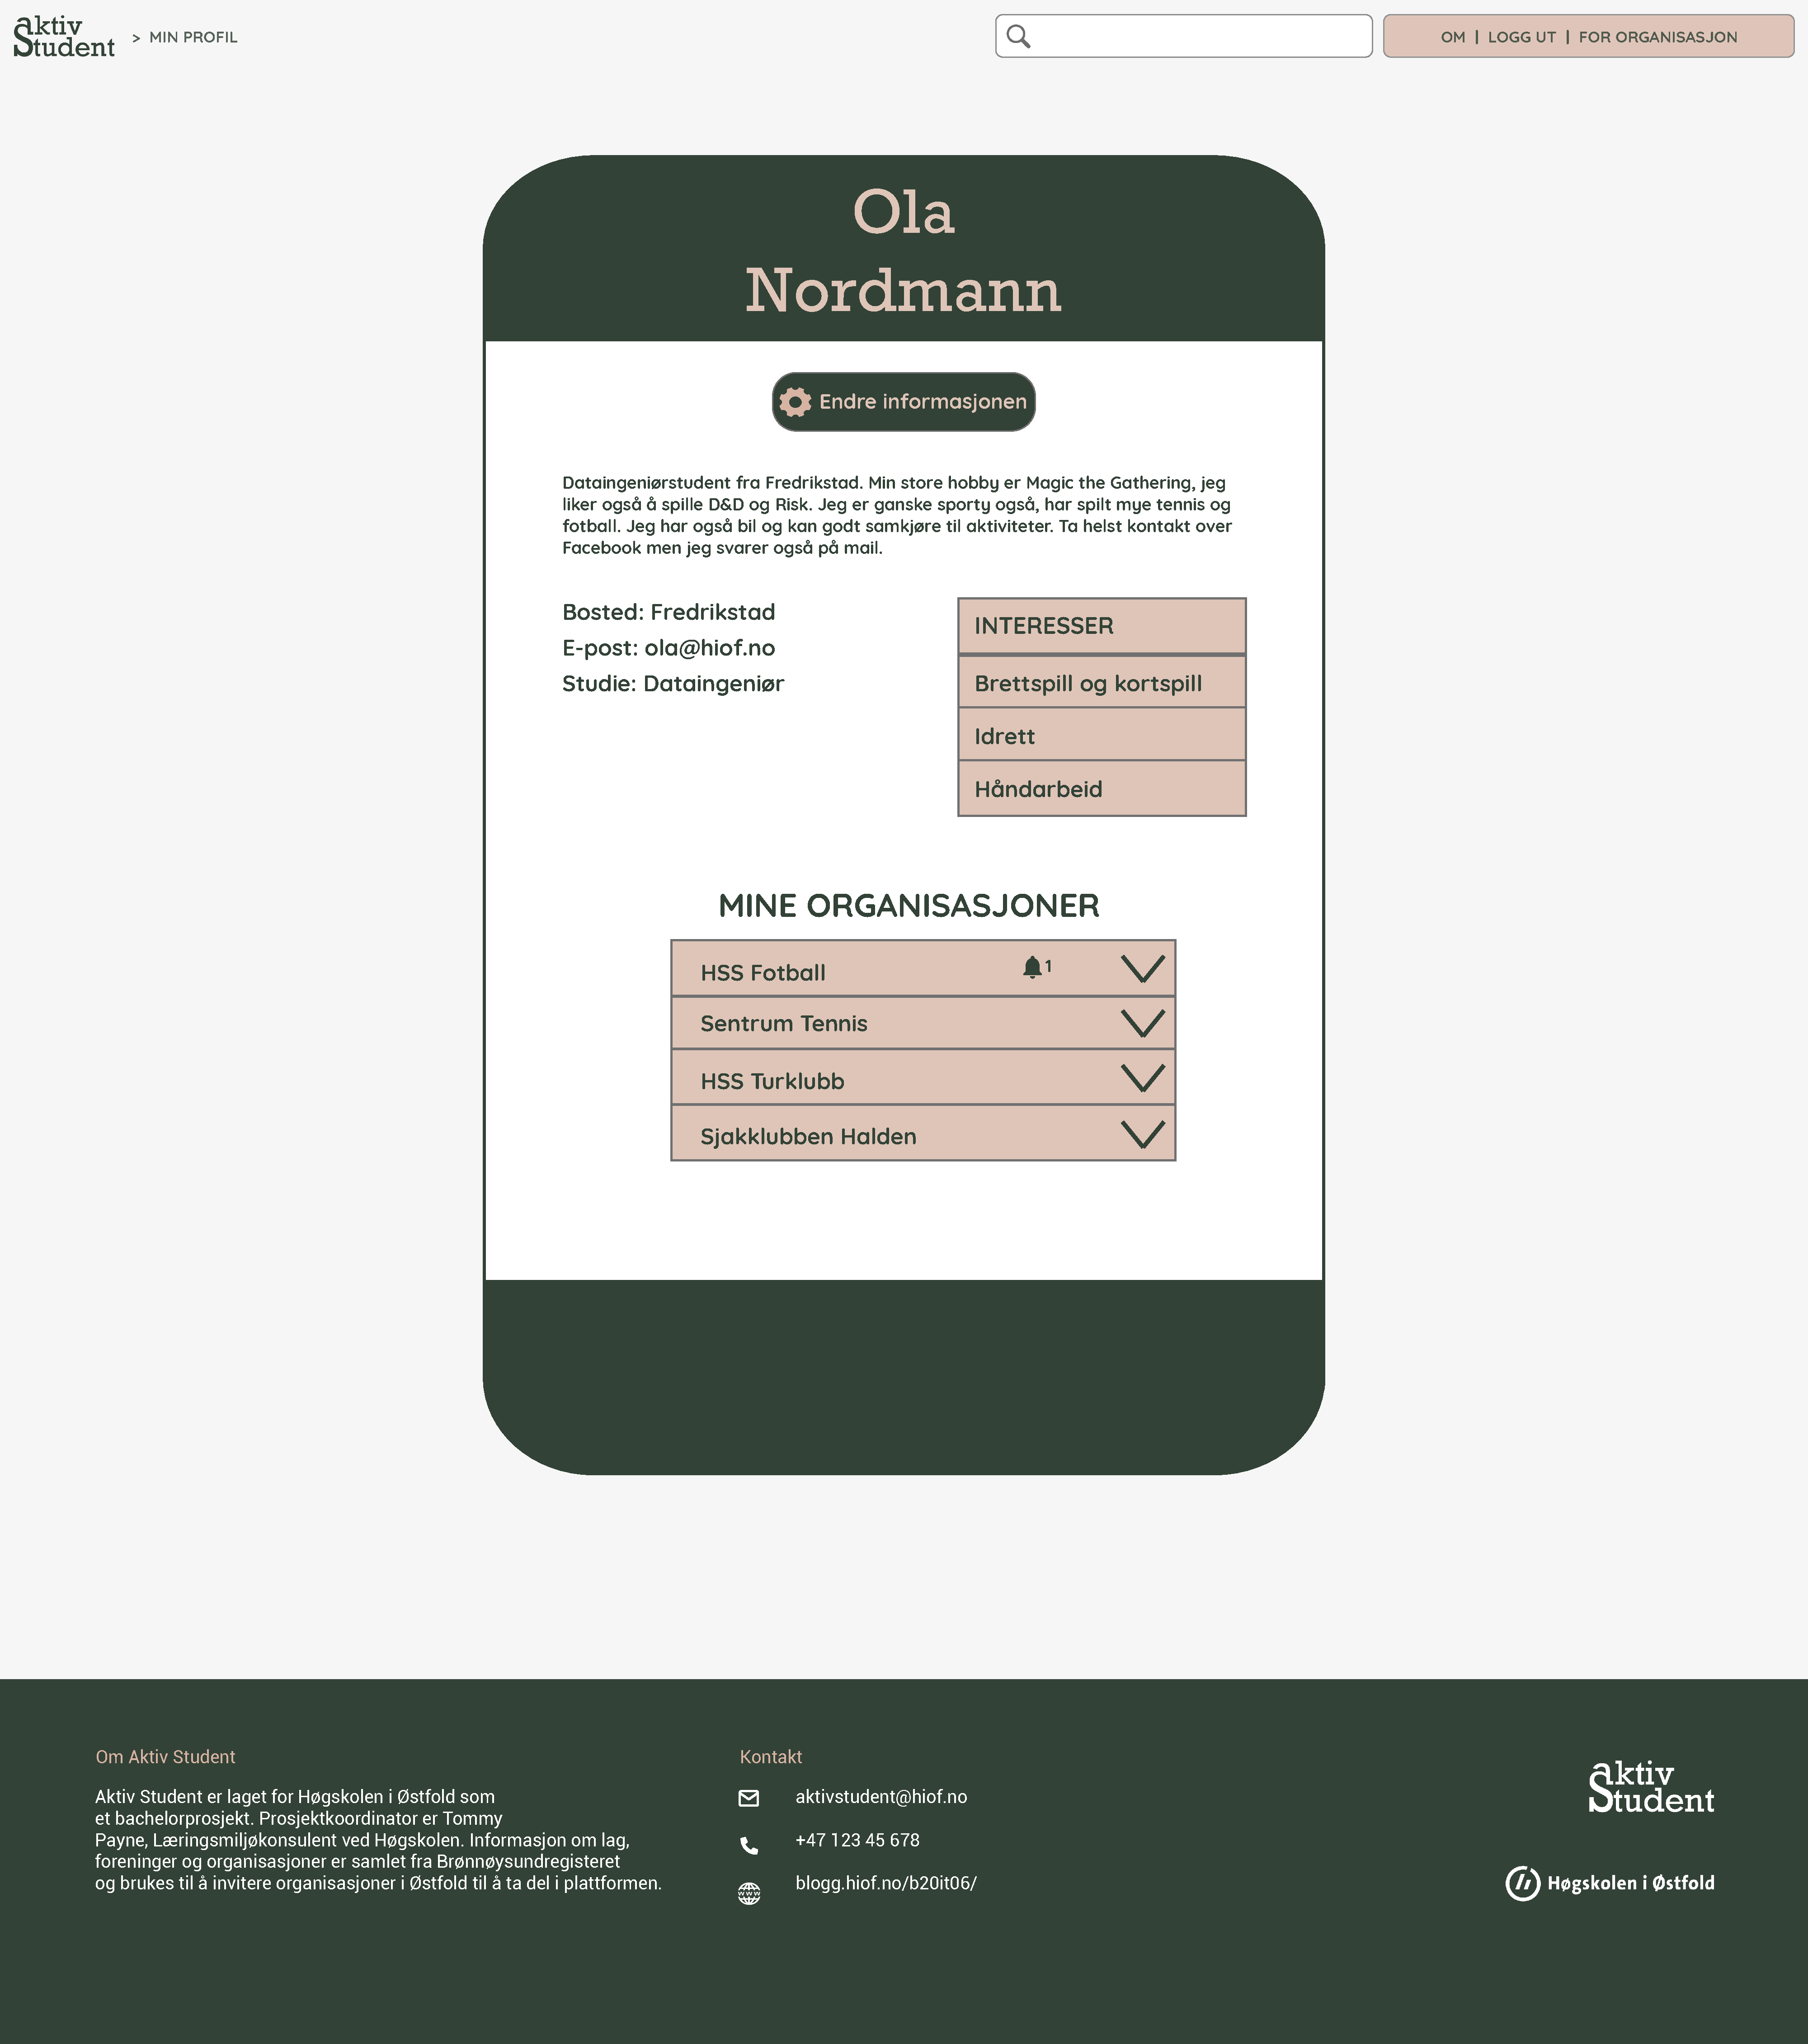
\includegraphics[width=\textwidth]{Illustrasjoner/Skisser-pdf/3.0/3-10-min-profil.pdf}
\caption{Adobe XD-skisse av hvordan en innlogget eksempelbruker ser sin egen profil}
\label{vedlegg:3-10-min-profil}
\end{figure}

\section{Om Aktiv Student}

\begin{figure}[H]
\centering

\includegraphics[width=\textwidth]{Illustrasjoner/Skisser-pdf/3.0/3-11-om-oss.pdf}
\caption{Adobe XD-skisse av {\em om}-siden til tjensten}
\label{vedlegg:3-11-om}
\end{figure}

\section{Kartleggingstest}

\begin{figure}[H]
\centering
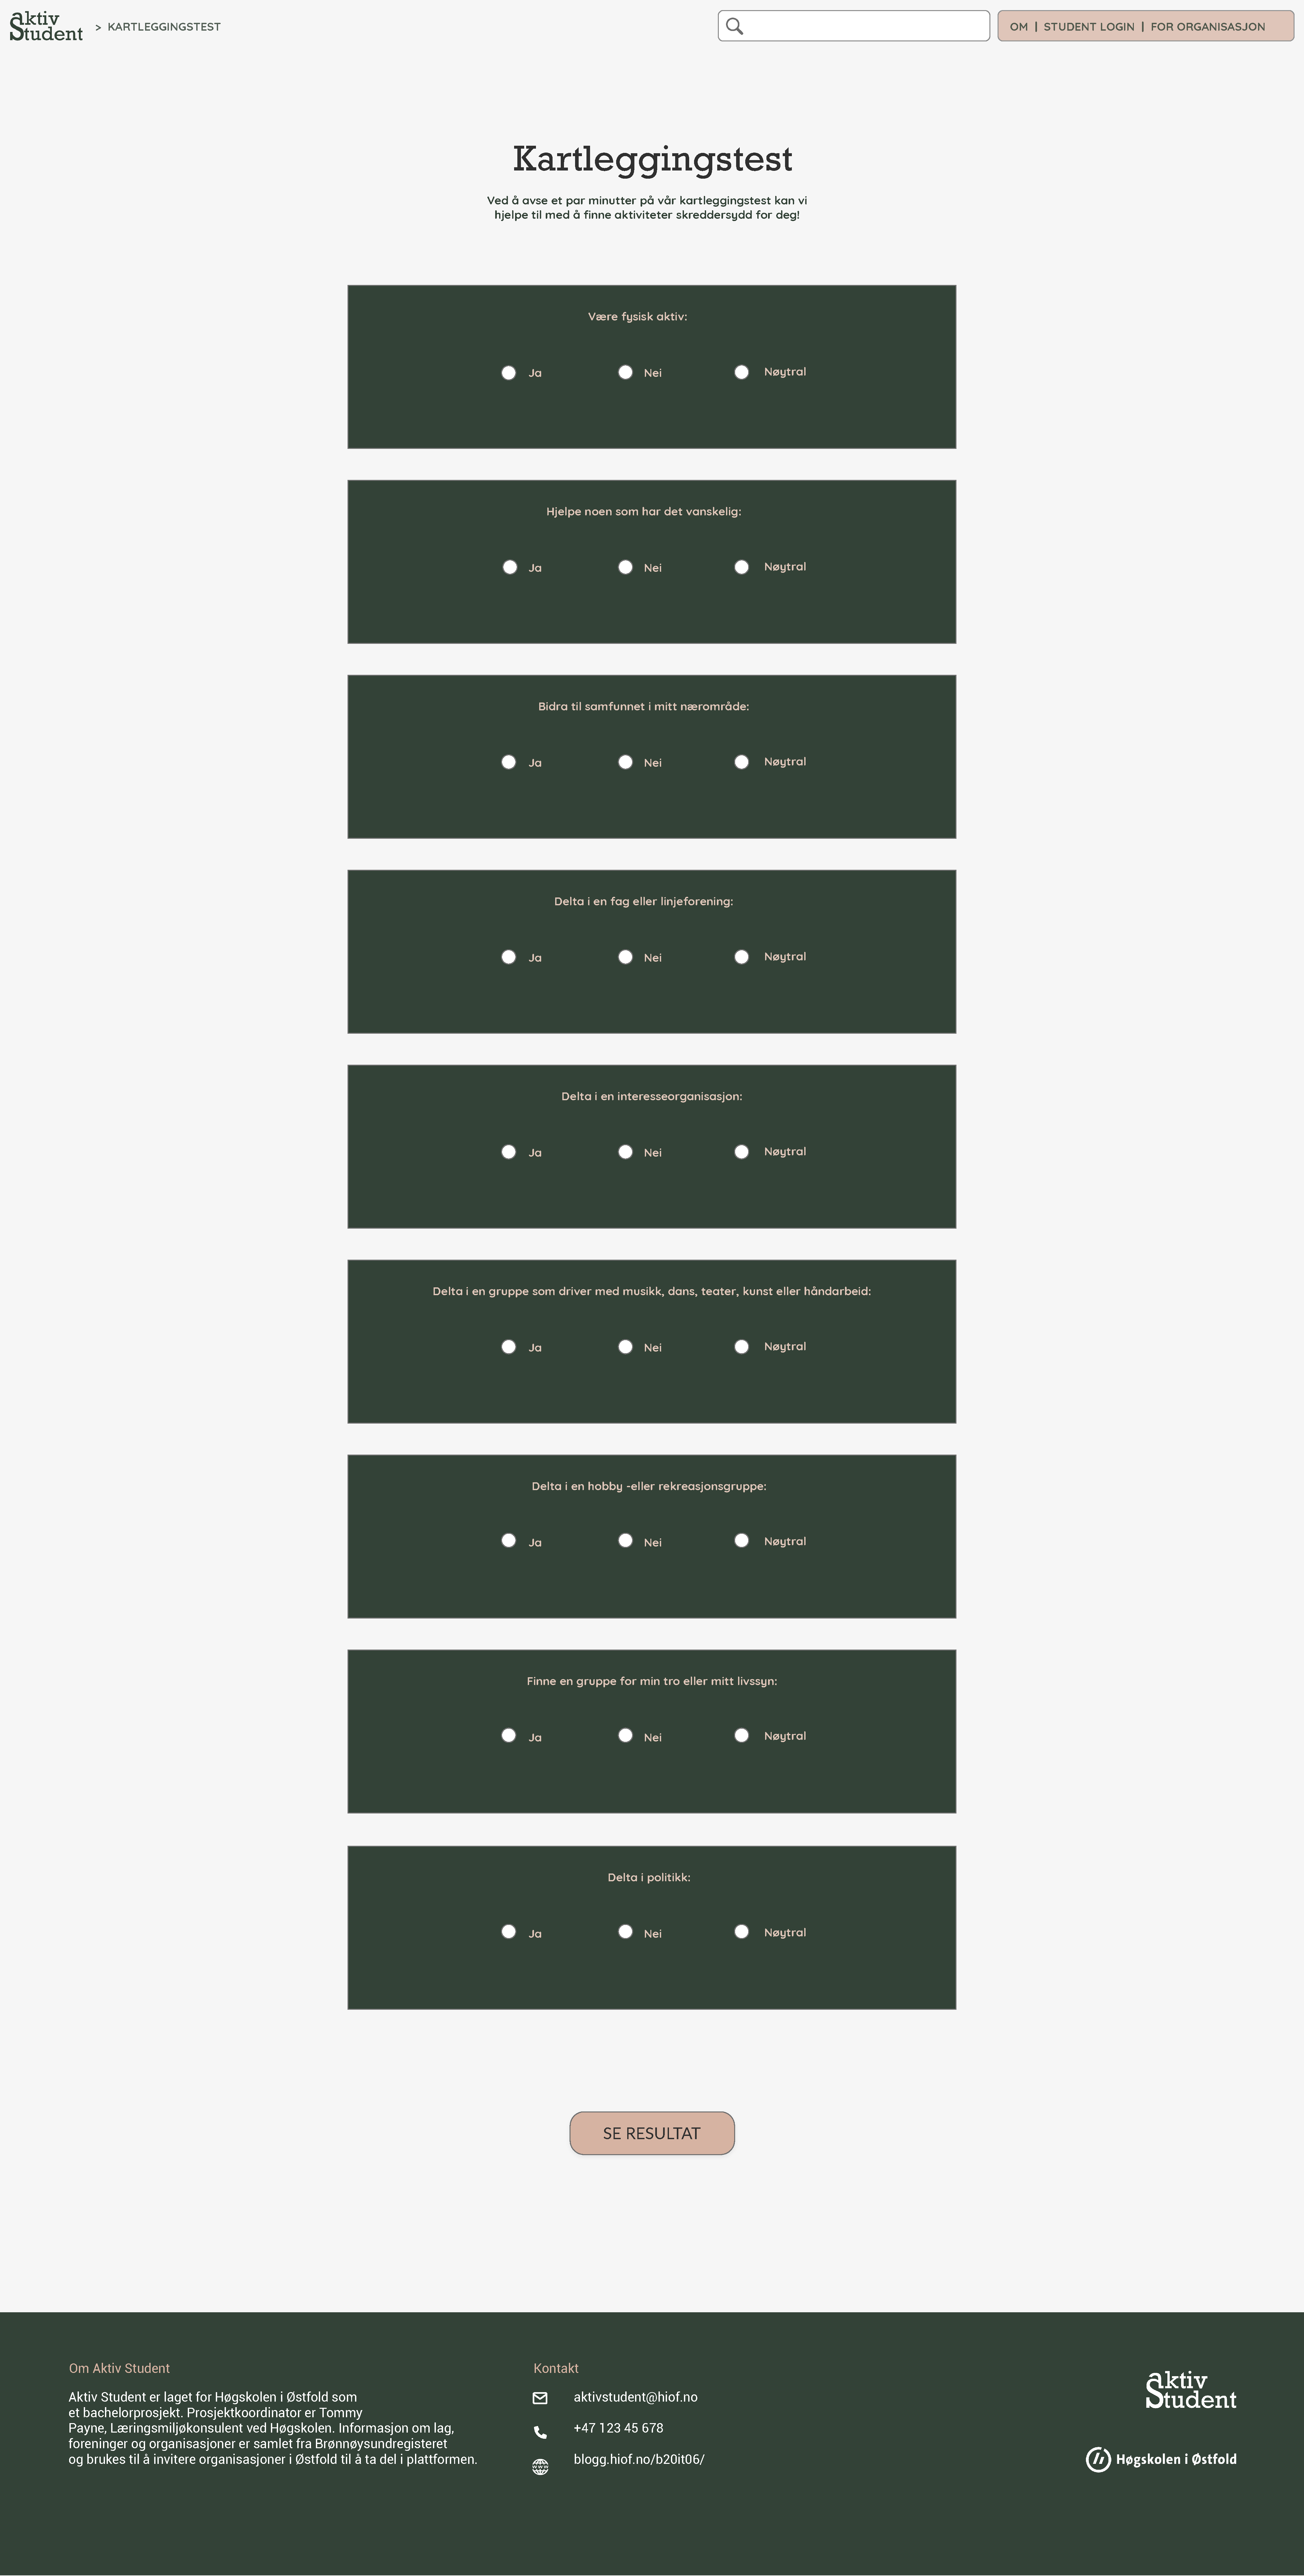
\includegraphics[width=.6\textwidth]{Illustrasjoner/Skisser-pdf/3.0/3-12-kartleggingstest.pdf}
\caption{Adobe XD-skisse av kartleggingstesten med eksempelspørsmål før noen av spørsmålene er besvart}
\label{vedlegg:3-12-kartlegging}
\end{figure}

\section{Kartleggingstest etter bruker har svart {\em ja} på første spørsmål}

\begin{figure}[H]
\centering
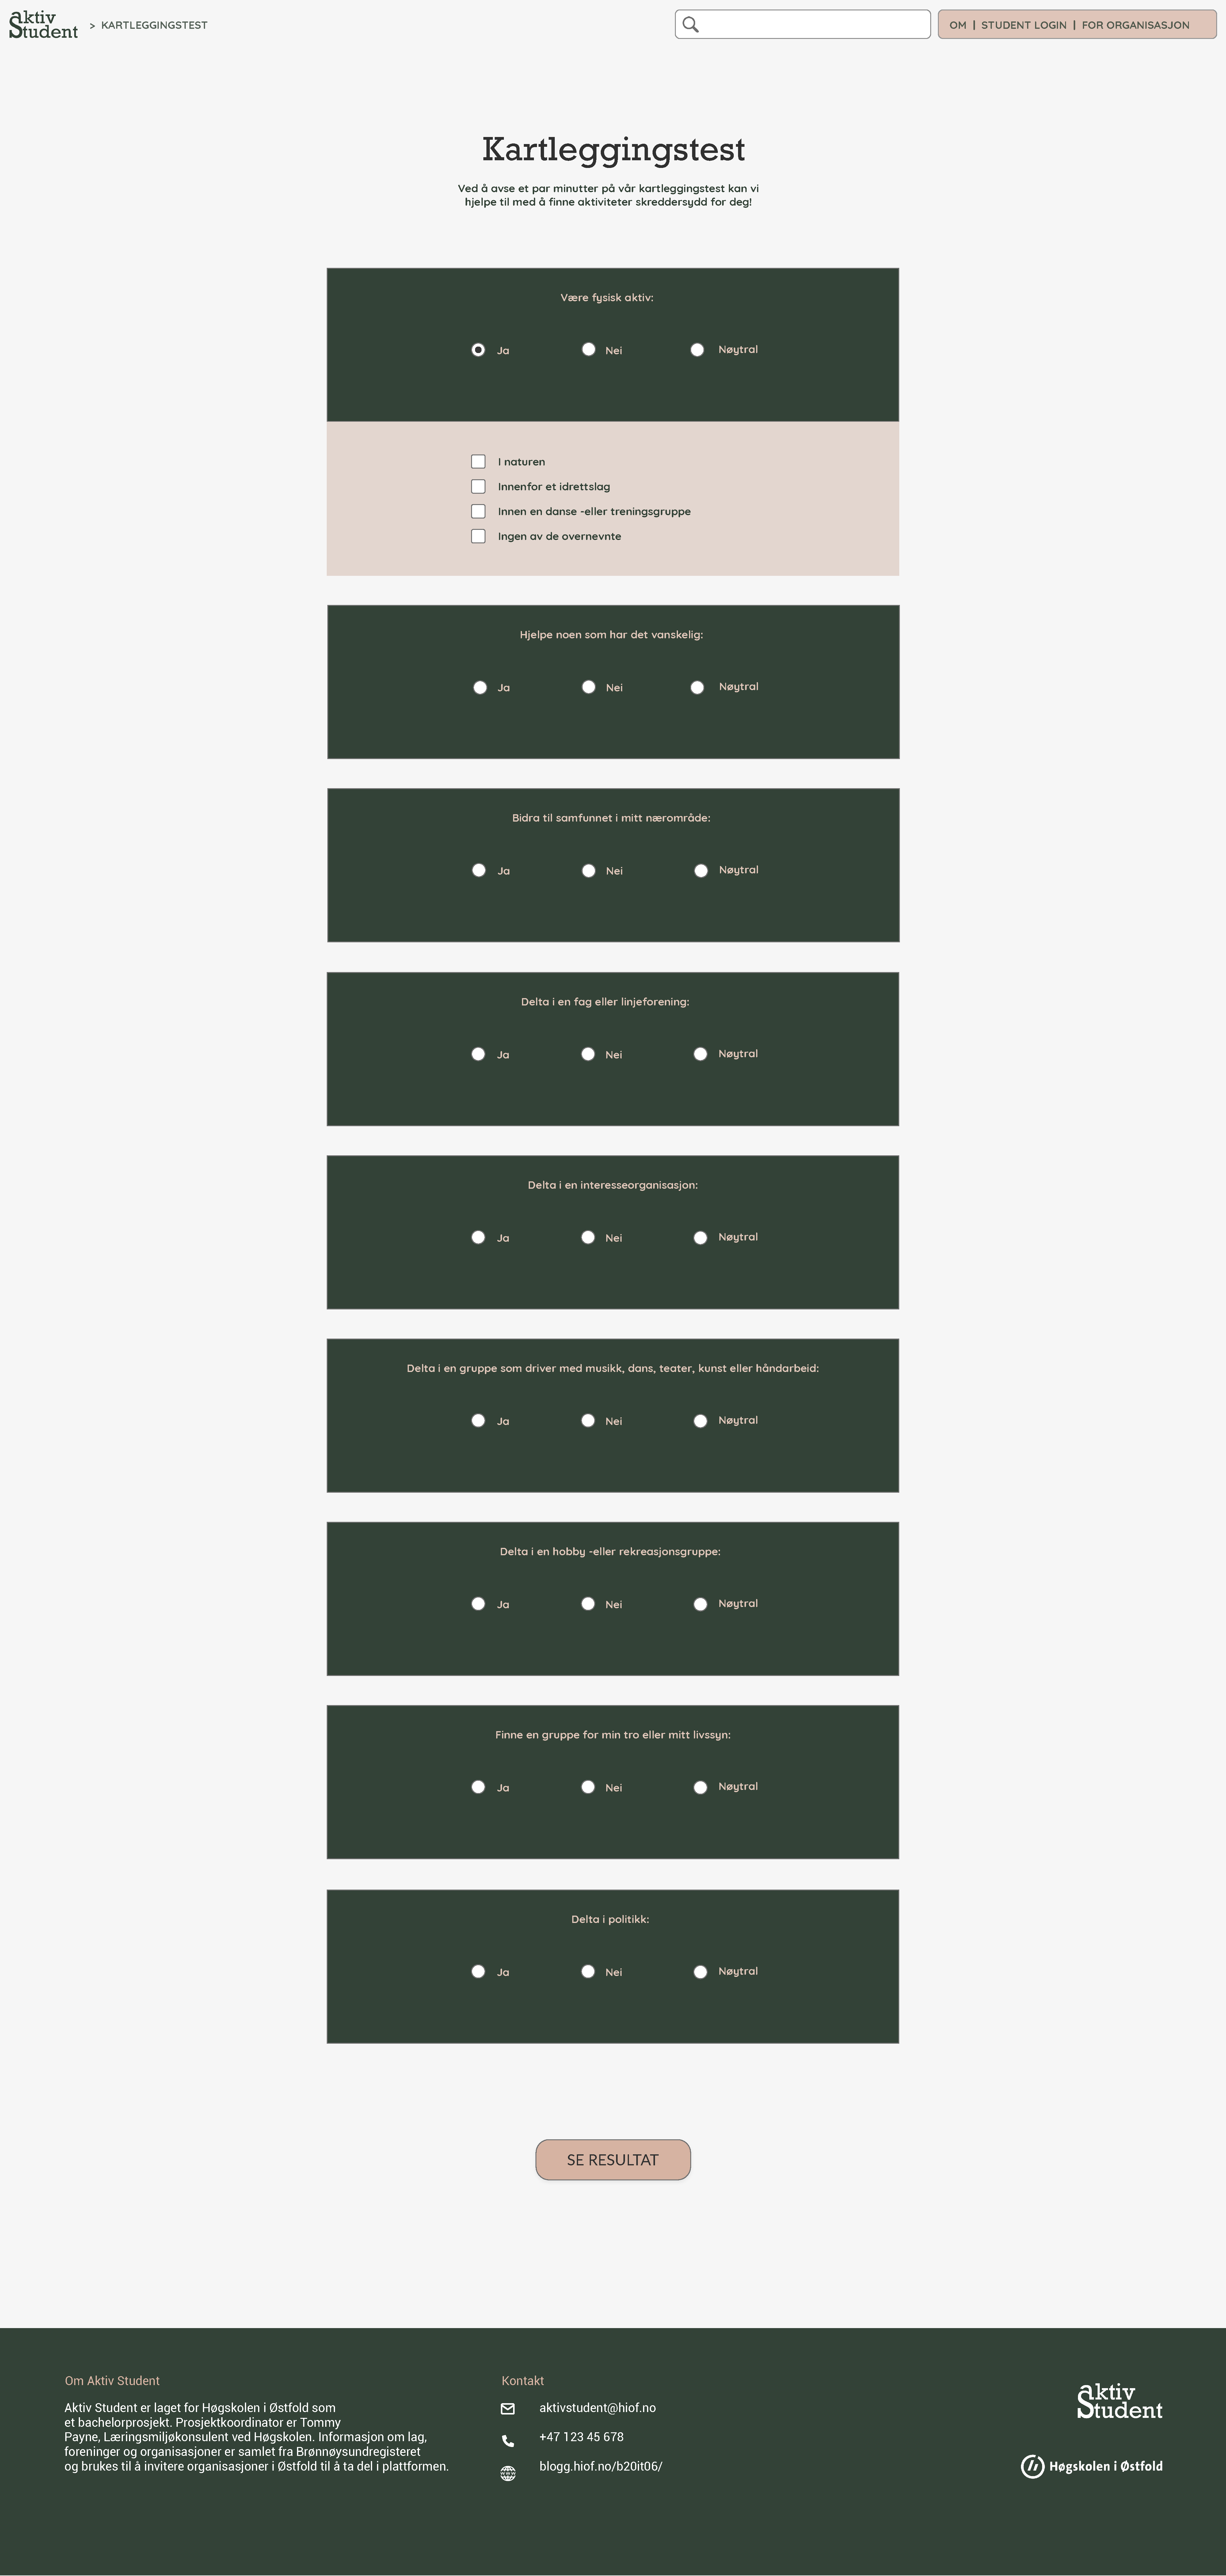
\includegraphics[width=.6\textwidth]{Illustrasjoner/Skisser-pdf/3.0/3-13-kartleggingstest-ved-svart-ja.pdf}
\caption{Adobe XD-skisse av kartleggingstesten med eksempelspørsmål etter bruker har svart {\em ja} på første spørsmål}
\label{vedlegg:3-13-kartlegging-svart-ja}
\end{figure}

\section{Resultater fra kartleggingstest}

\begin{figure}[H]
\centering
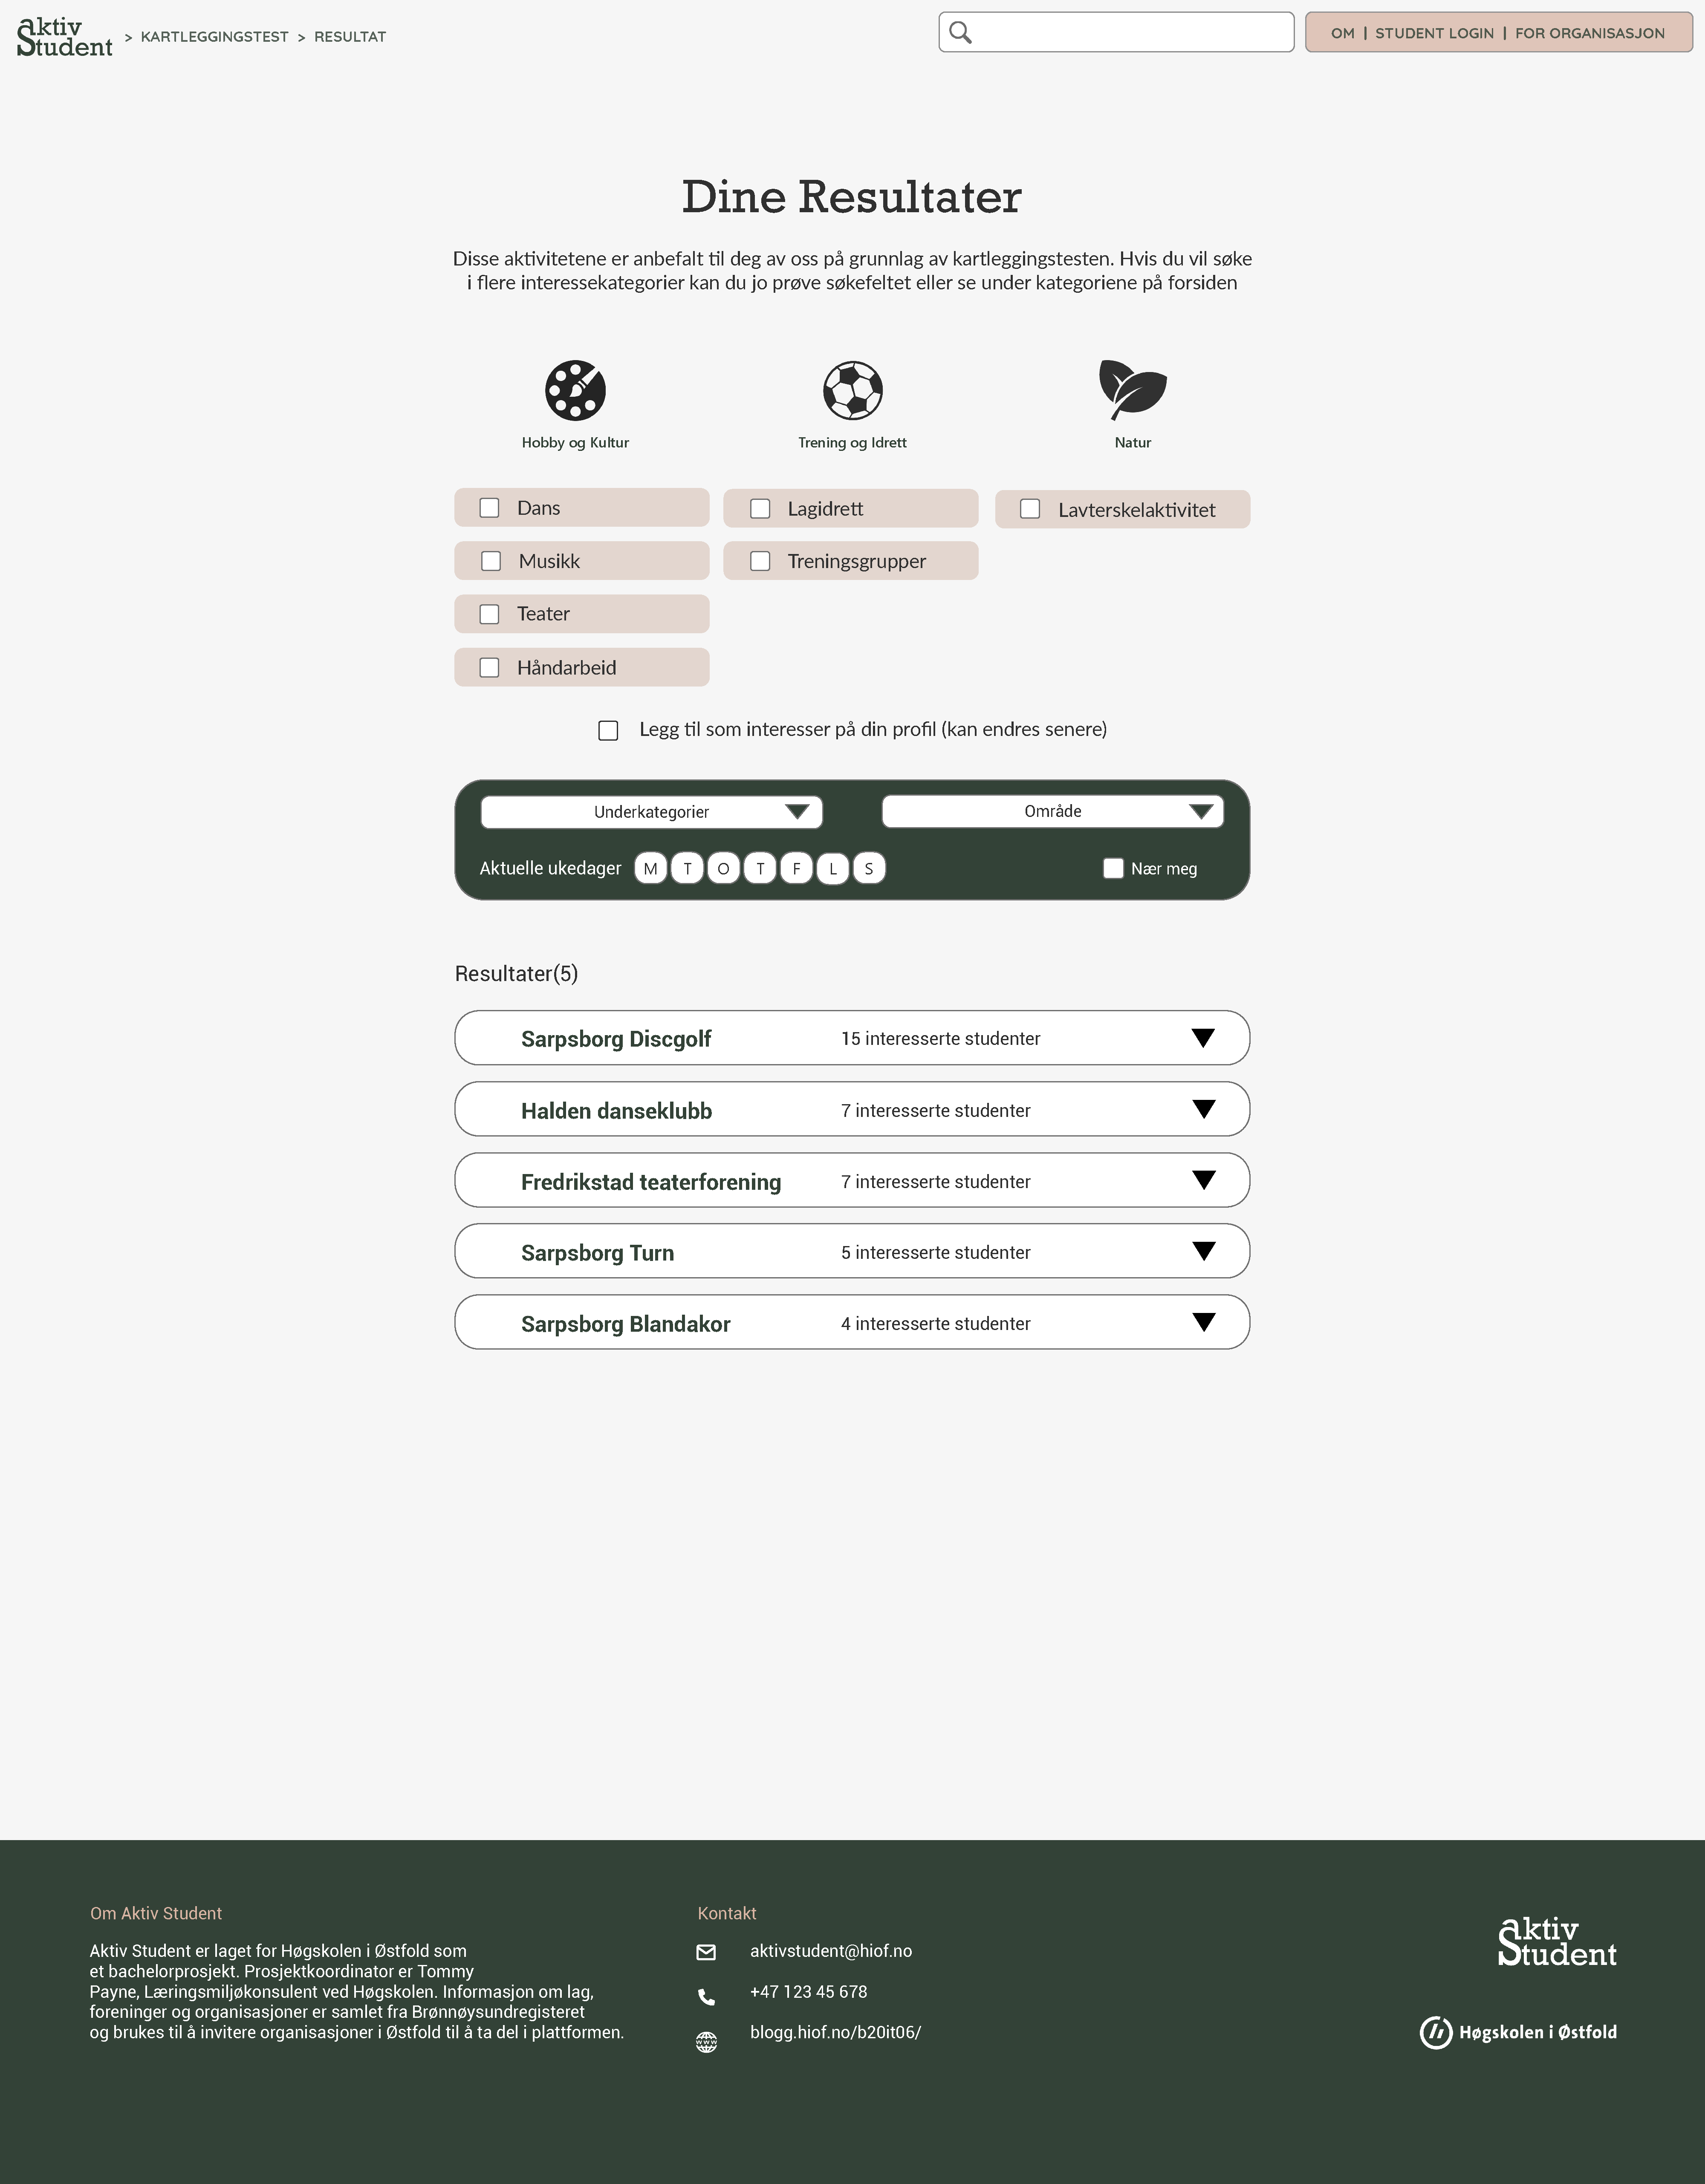
\includegraphics[width=\textwidth]{Illustrasjoner/Skisser-pdf/3.0/3-14-kartleggingstest-resultat.pdf}
\caption{Adobe XD-skisse av av resultatsiden fra kartleggingstesten}
\label{vedlegg:3-14-resultat-kartlegging}
\end{figure}

\section{Innlogging for organisasjoner}

\begin{figure}[H]
\centering
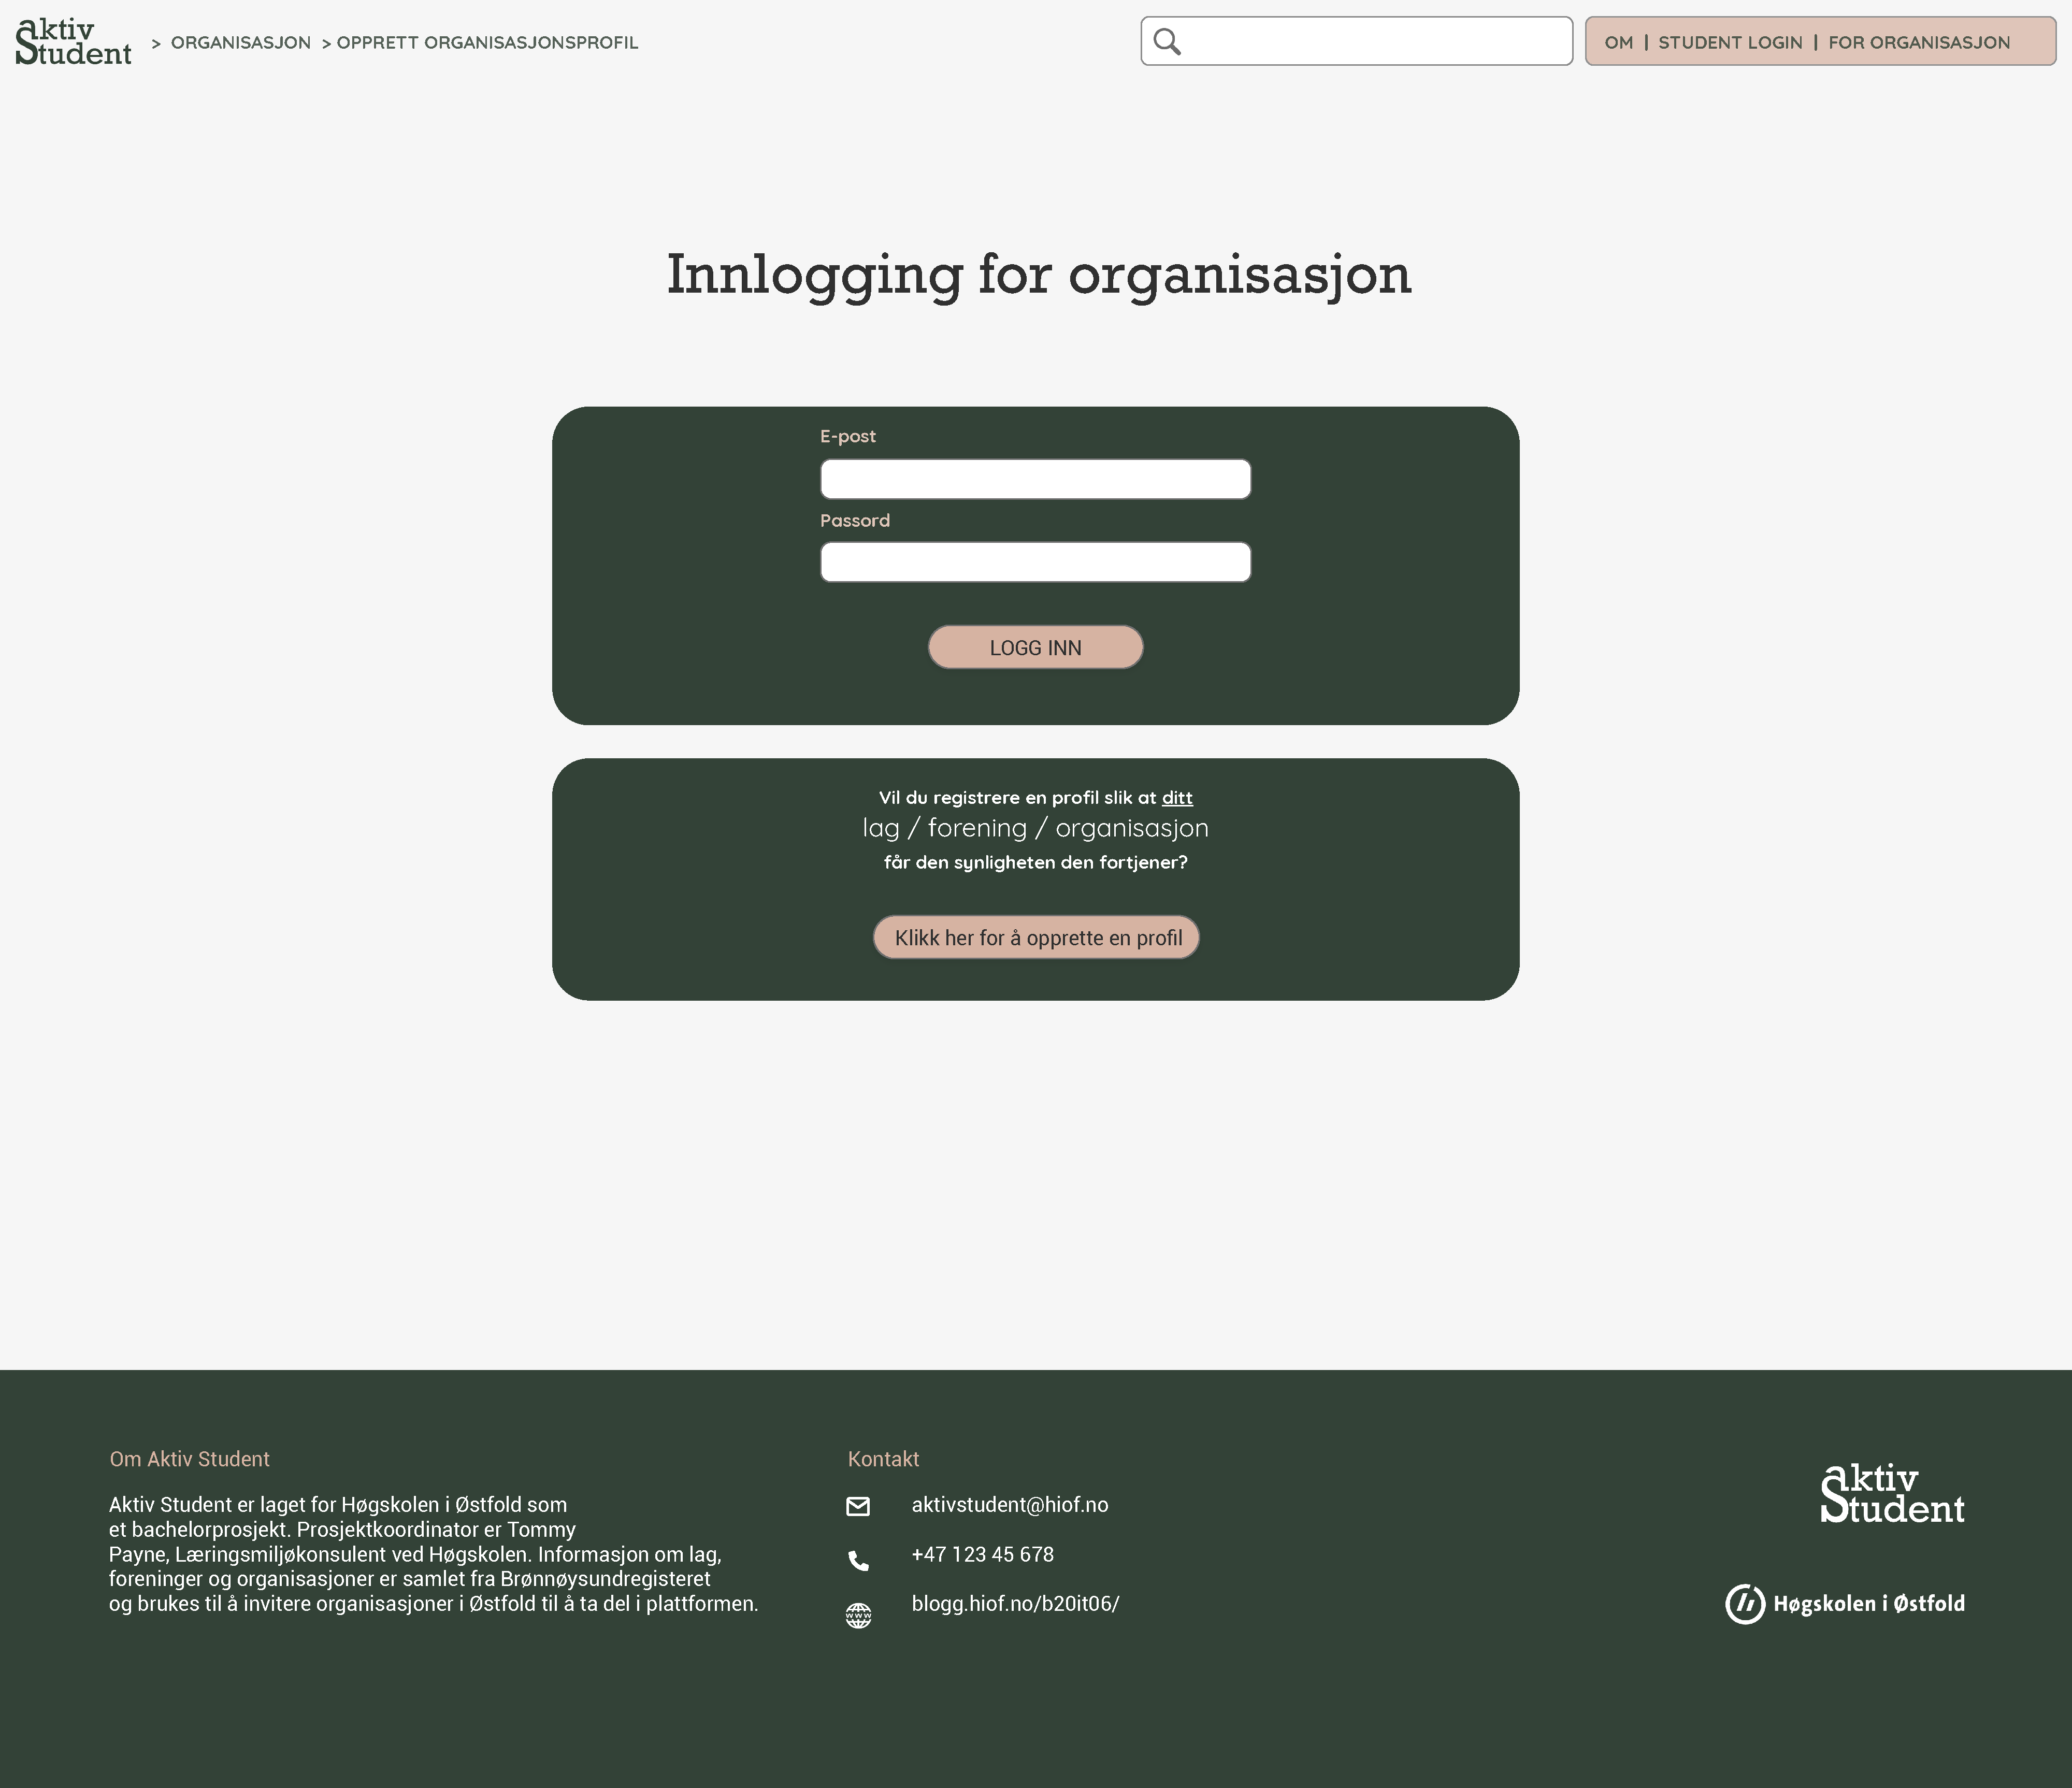
\includegraphics[width=\textwidth]{Illustrasjoner/Skisser-pdf/3.0/3-15-innlogging-organisasjon.pdf}
\caption{Adobe XD-skisse av innloggingsiden for organisasjoner}
\label{vedlegg:3-15-innlogging-org}
\end{figure}

\section{Opprett organisasjonsprofil}

\begin{figure}[H]
\centering
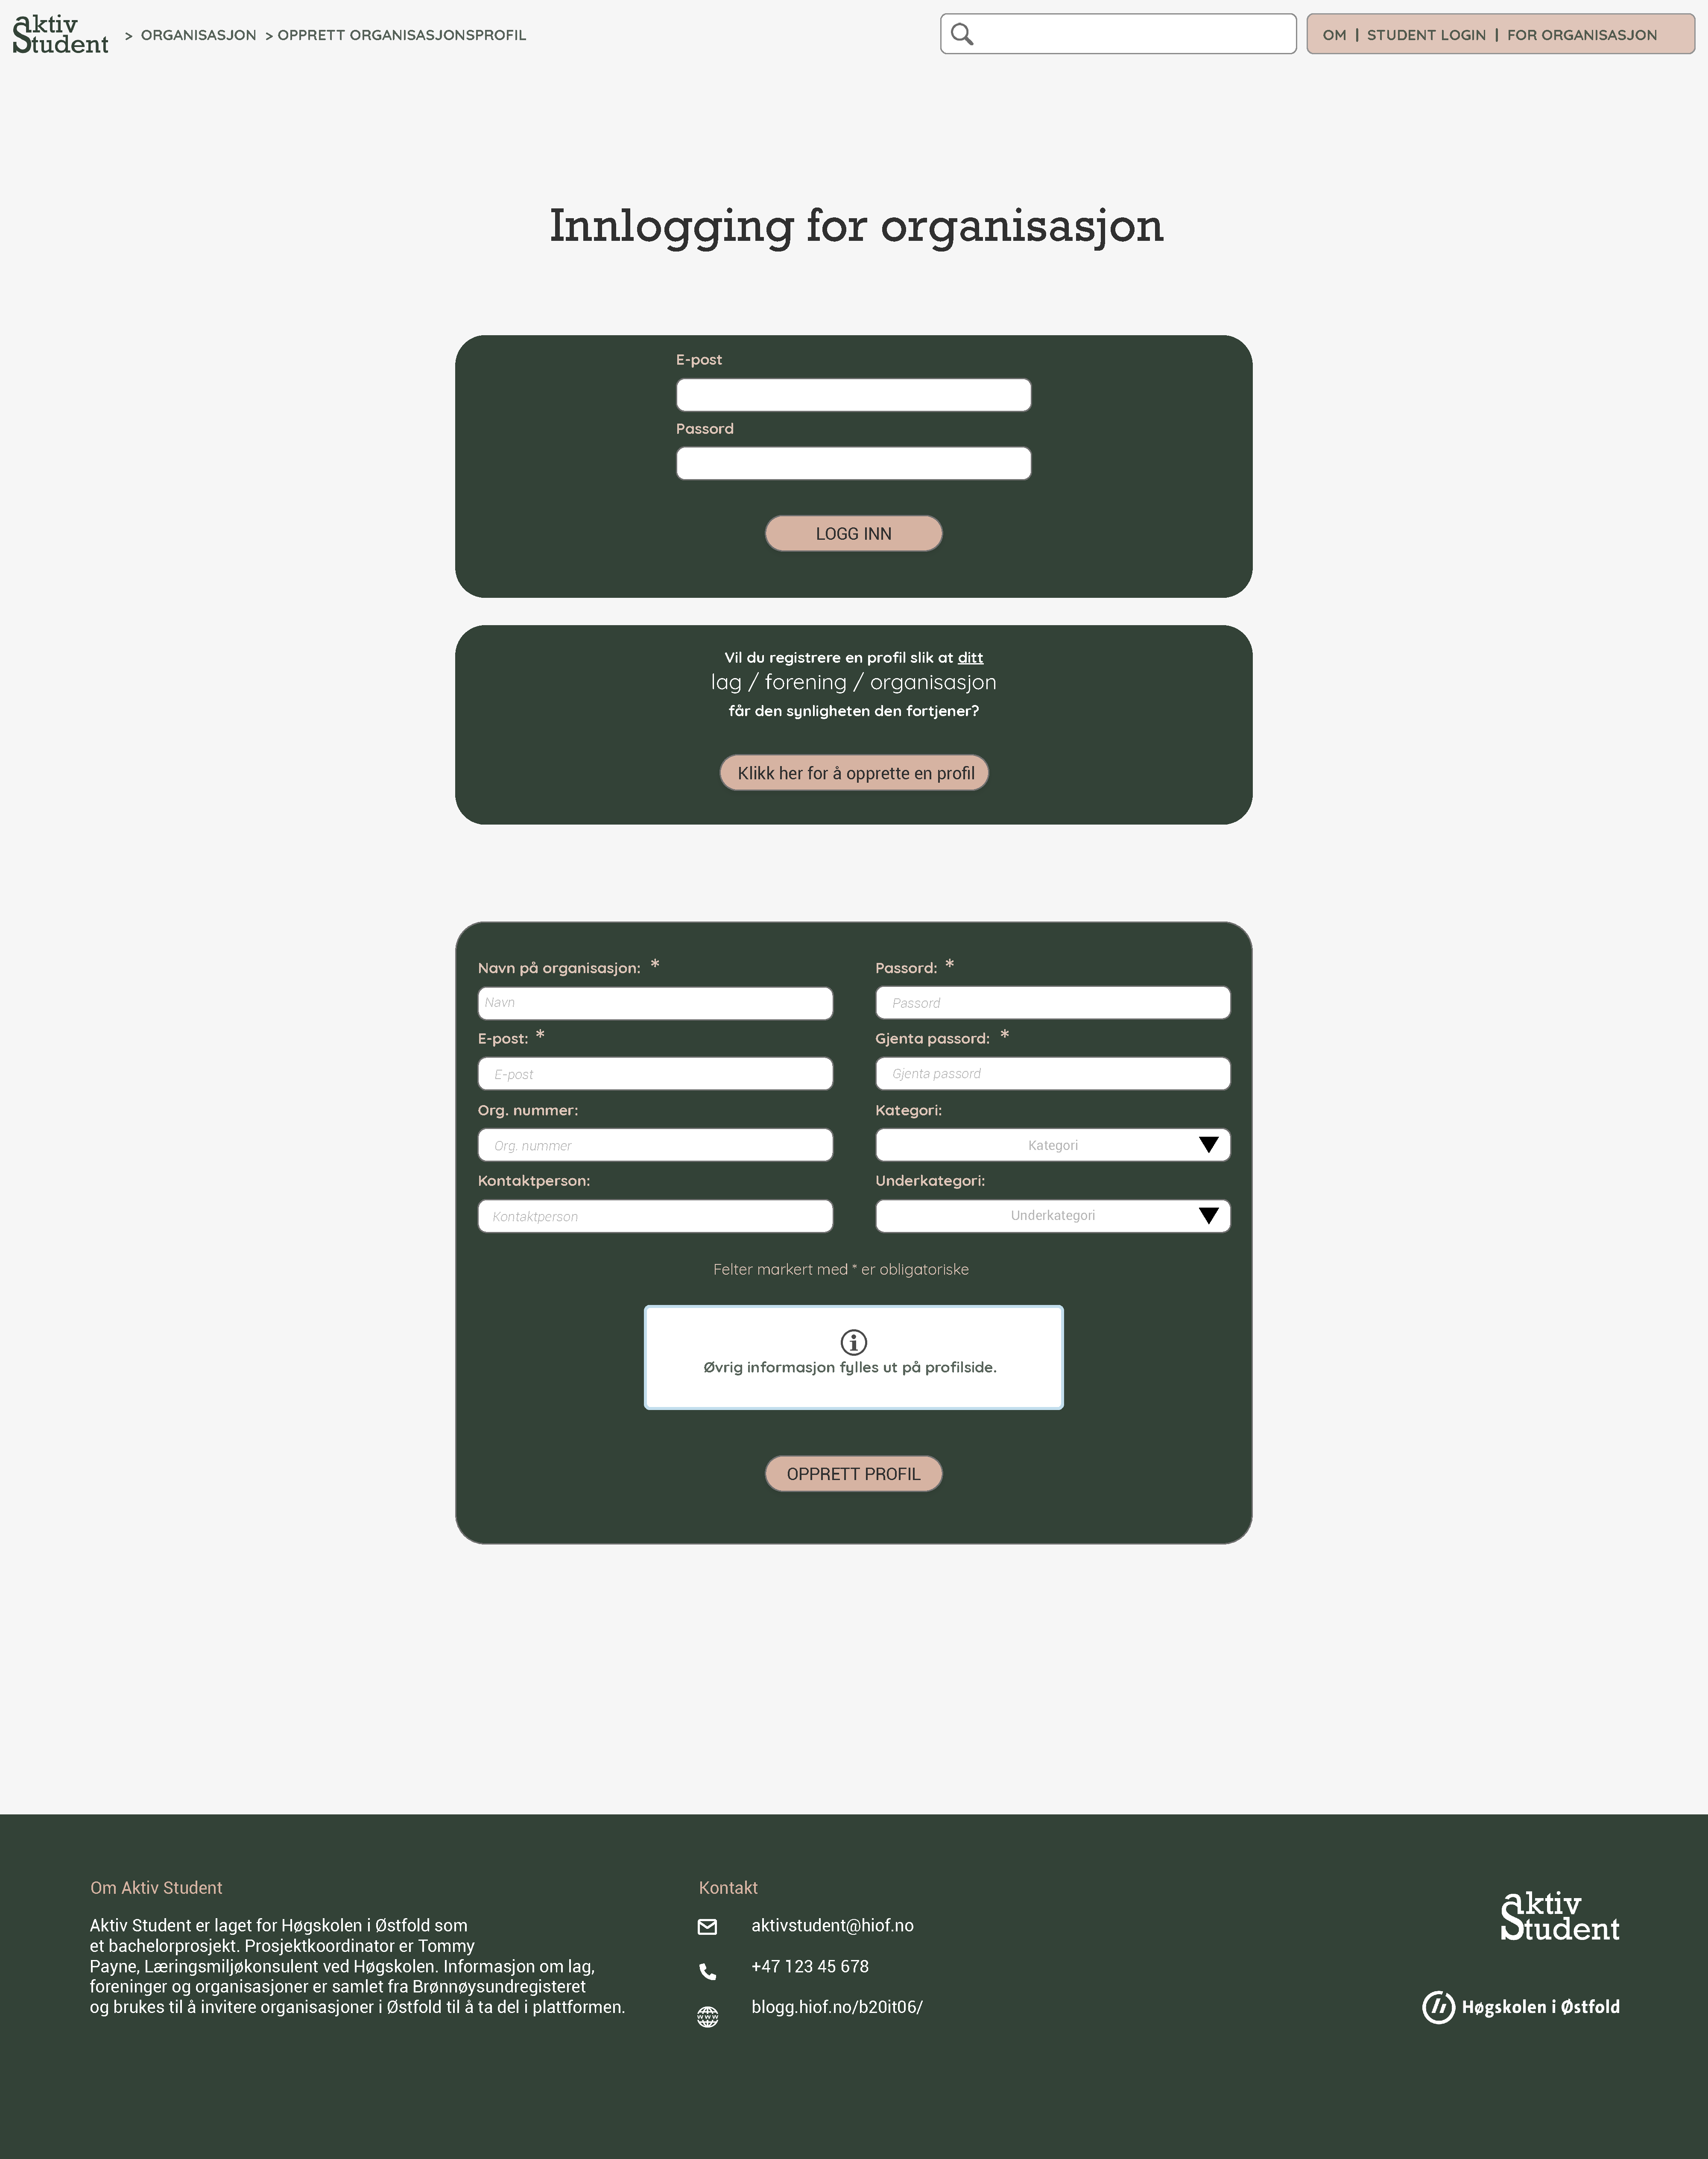
\includegraphics[width=\textwidth]{Illustrasjoner/Skisser-pdf/3.0/3-16-opprett-organisasjonsprofil.pdf}
\caption{Adobe XD-skisse av siden for å opprette organisasjonsprofil}
\label{vedlegg:3-16-opprett-orgprofil}
\end{figure}

\section{Innlogget organisasjonsprofil}

\begin{figure}[H]
\centering
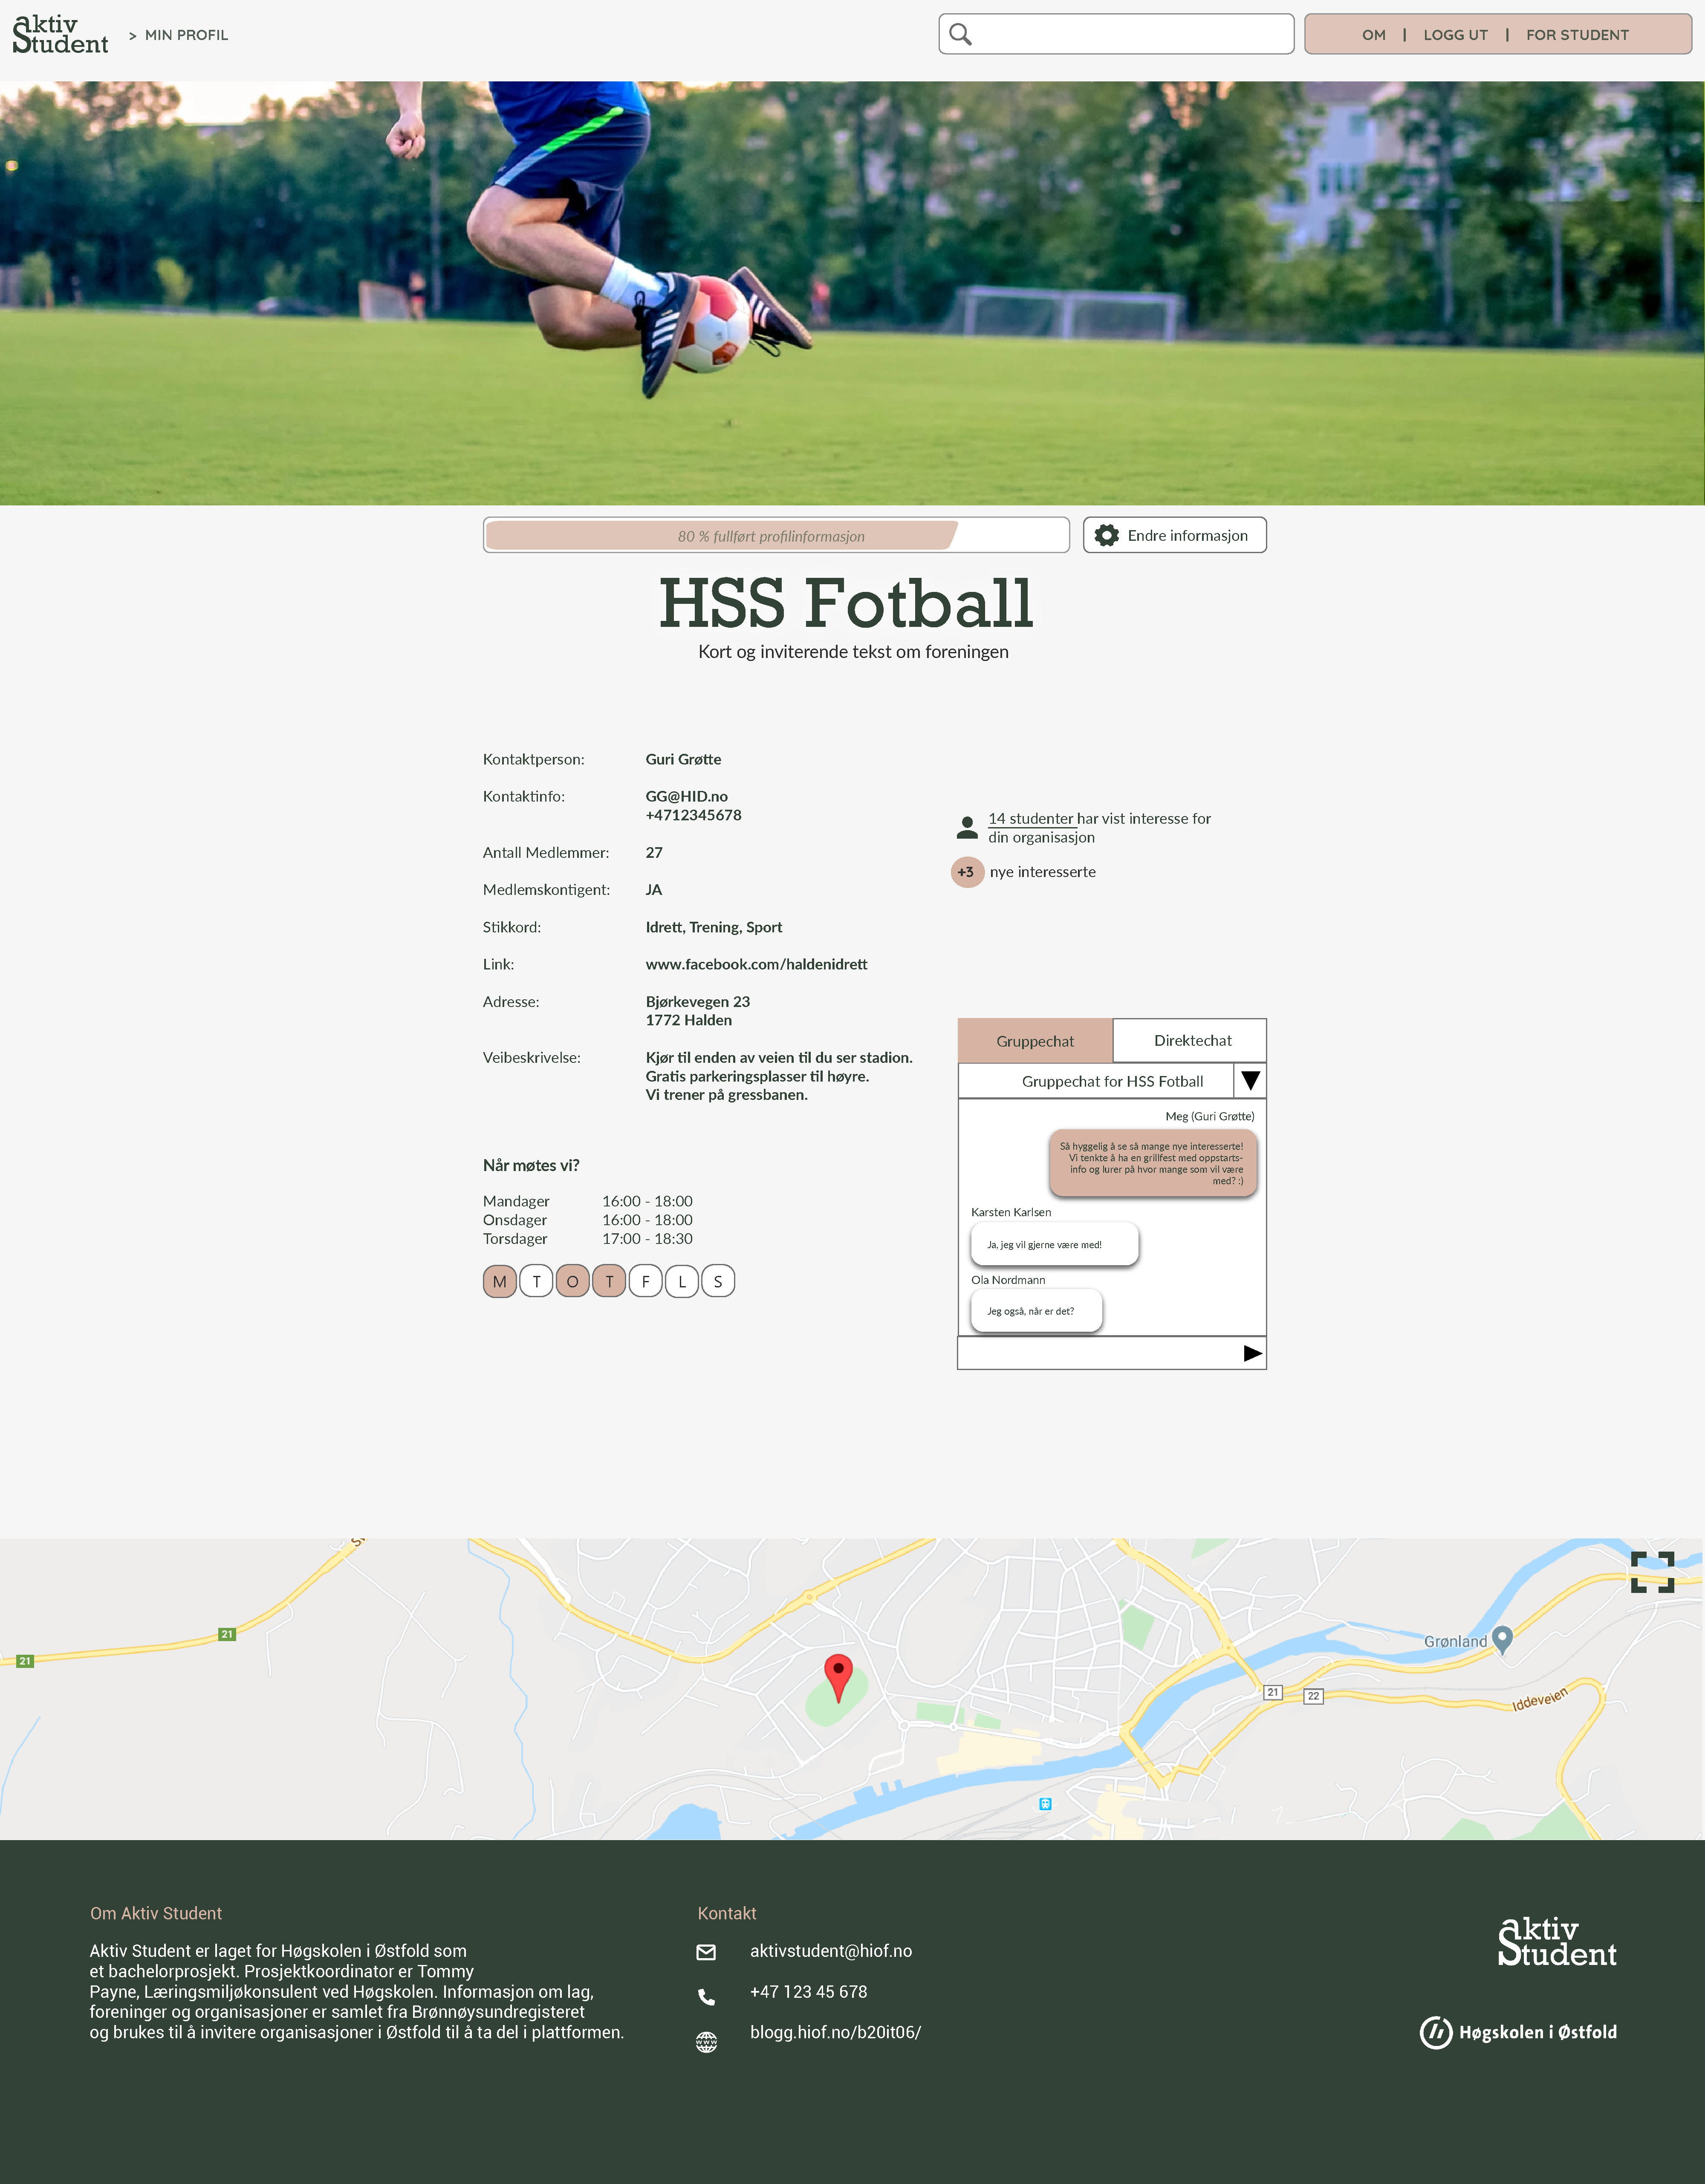
\includegraphics[width=\textwidth]{Illustrasjoner/Skisser-pdf/3.0/3-17-innlogget-organisasjon.pdf}
\caption{Adobe XD-skisse av hvordan eksempelorganisasjonen ser sin egen profil etter innlogging}
\label{vedlegg:3-17-innlogget-org}
\end{figure}

\section{Endre informasjon på innlogget organisasjonsprofil}

\begin{figure}[H]
\centering
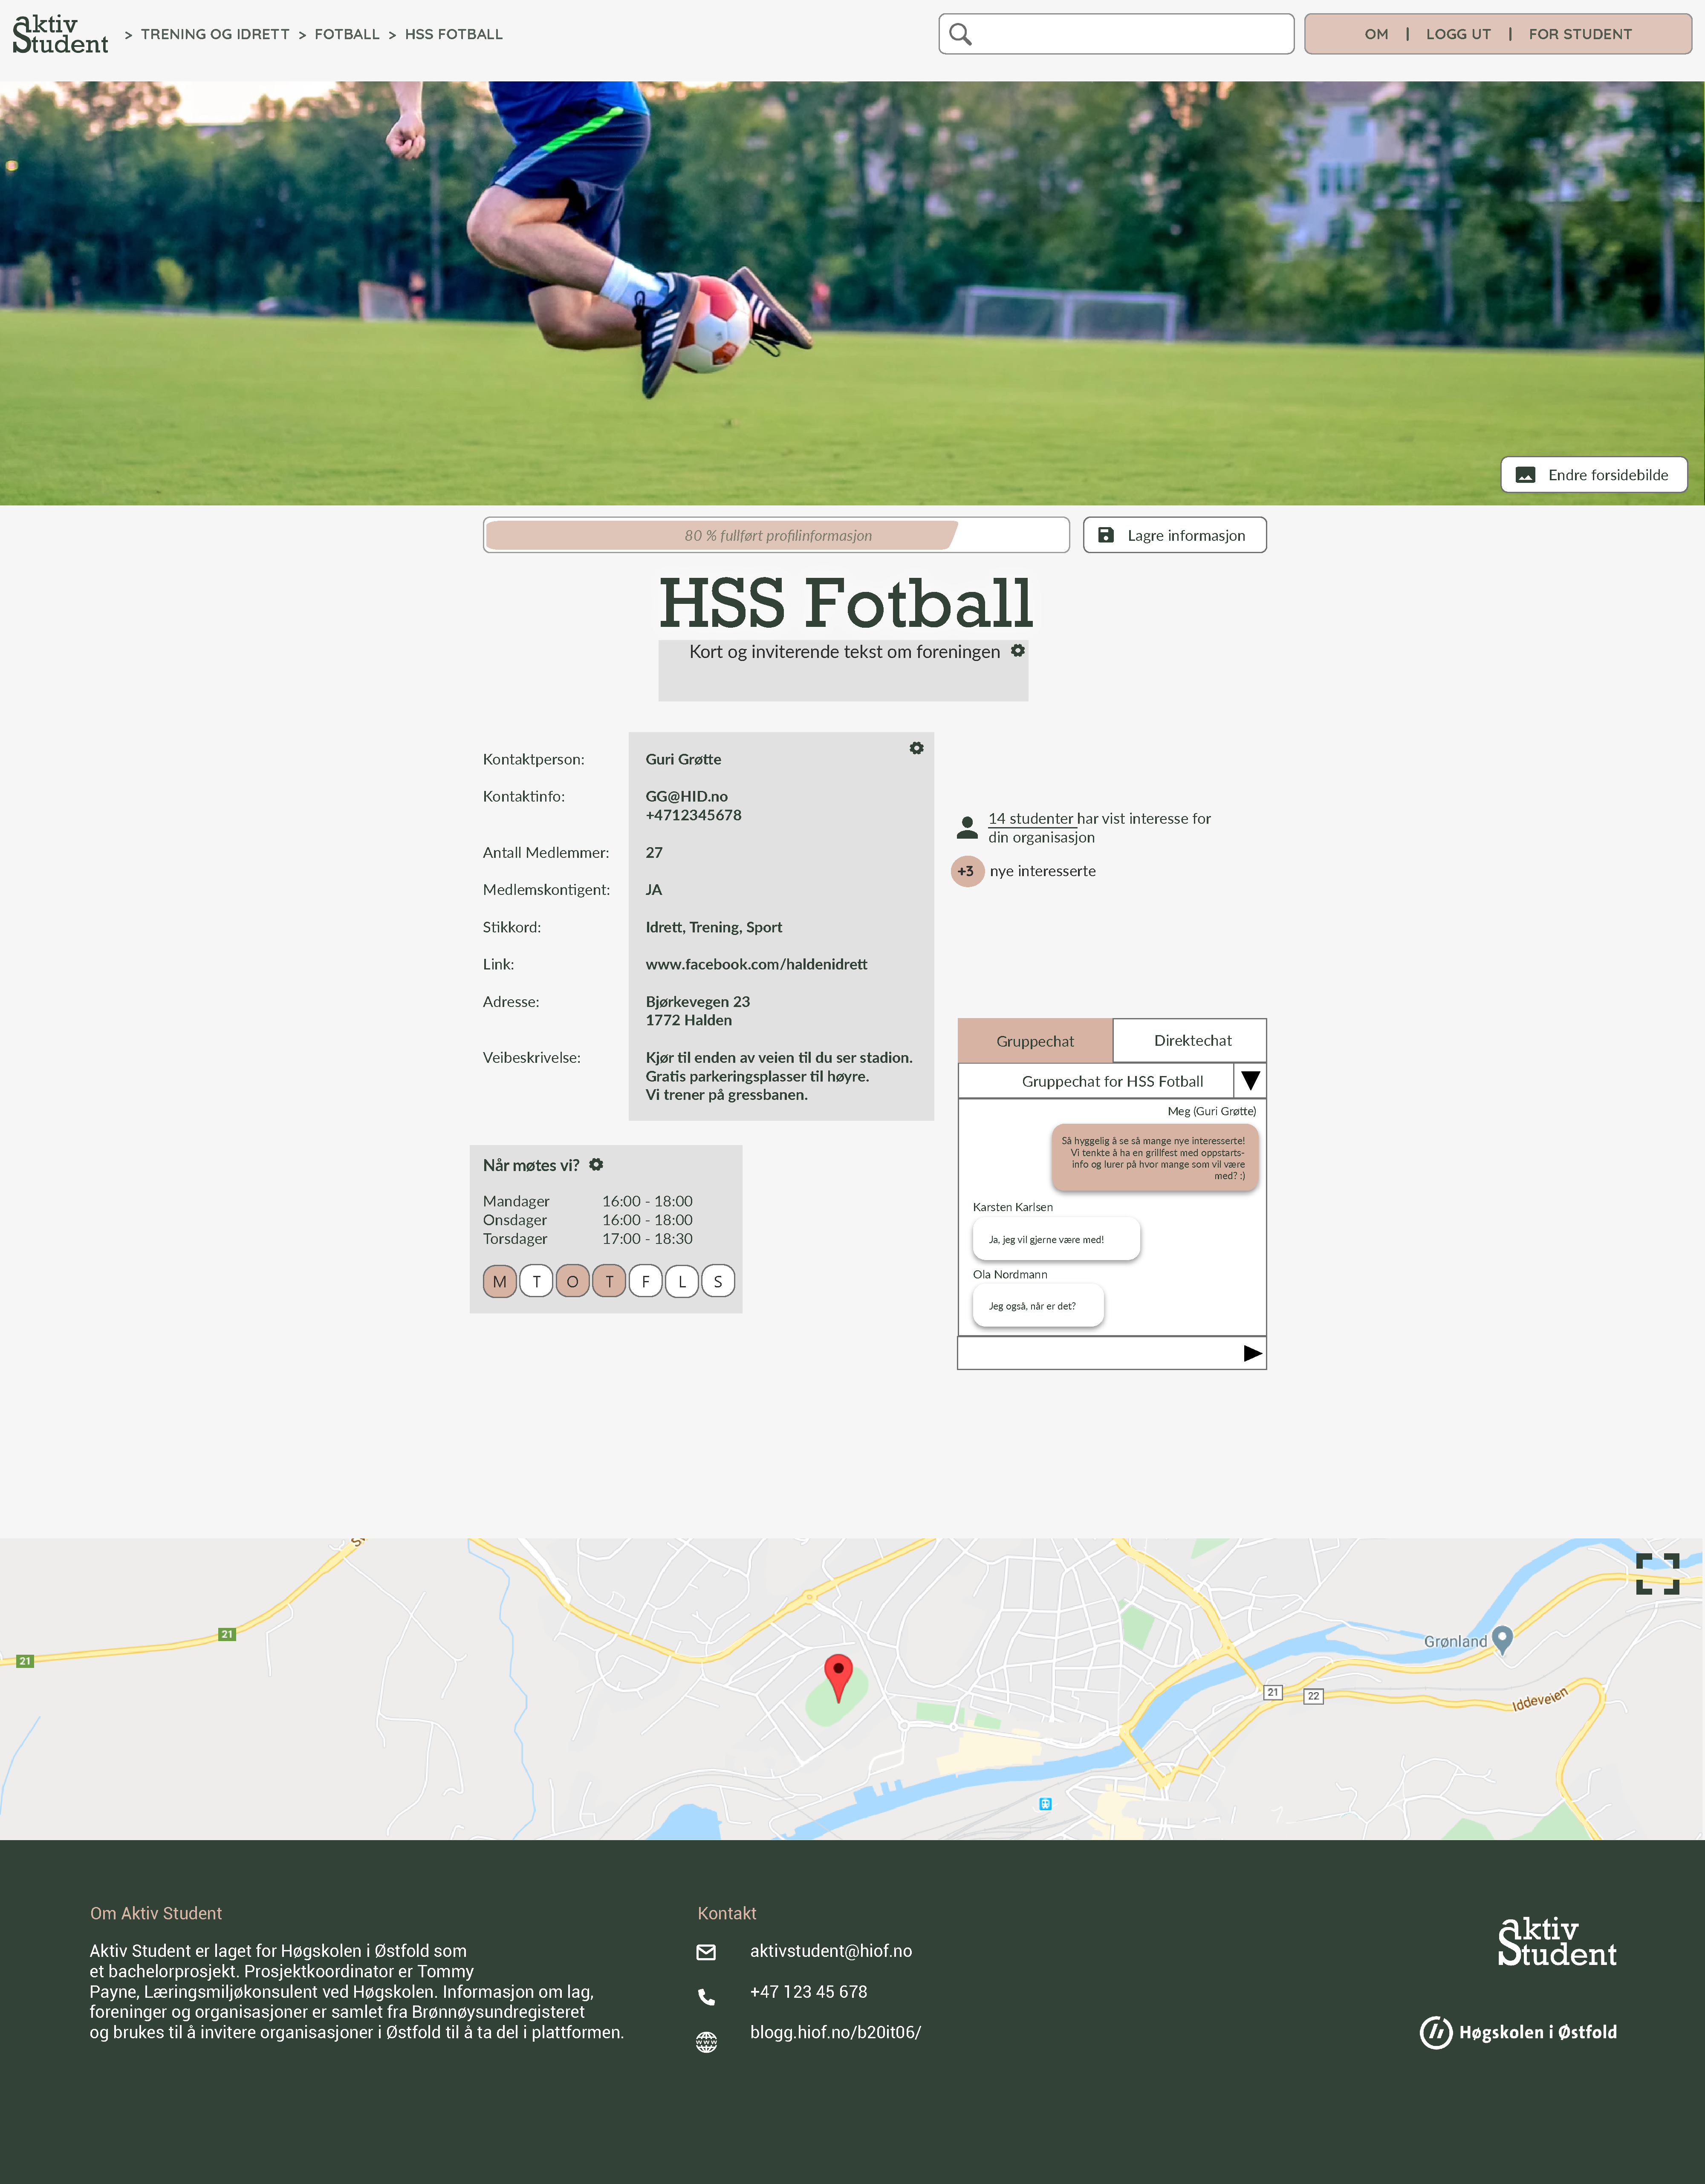
\includegraphics[width=\textwidth]{Illustrasjoner/Skisser-pdf/3.0/3-18-endre-info-organisasjon.pdf}
\caption{Adobe XD-skisse av hvordan eksempelorganisasjonen ser sin egen profil etter å ha trykket på {\em endre}-knappen}
\label{vedlegg:3-18-endre-info-org}
\end{figure}

\section{Administratorpanel oversikt}

\begin{figure}[H]
\centering
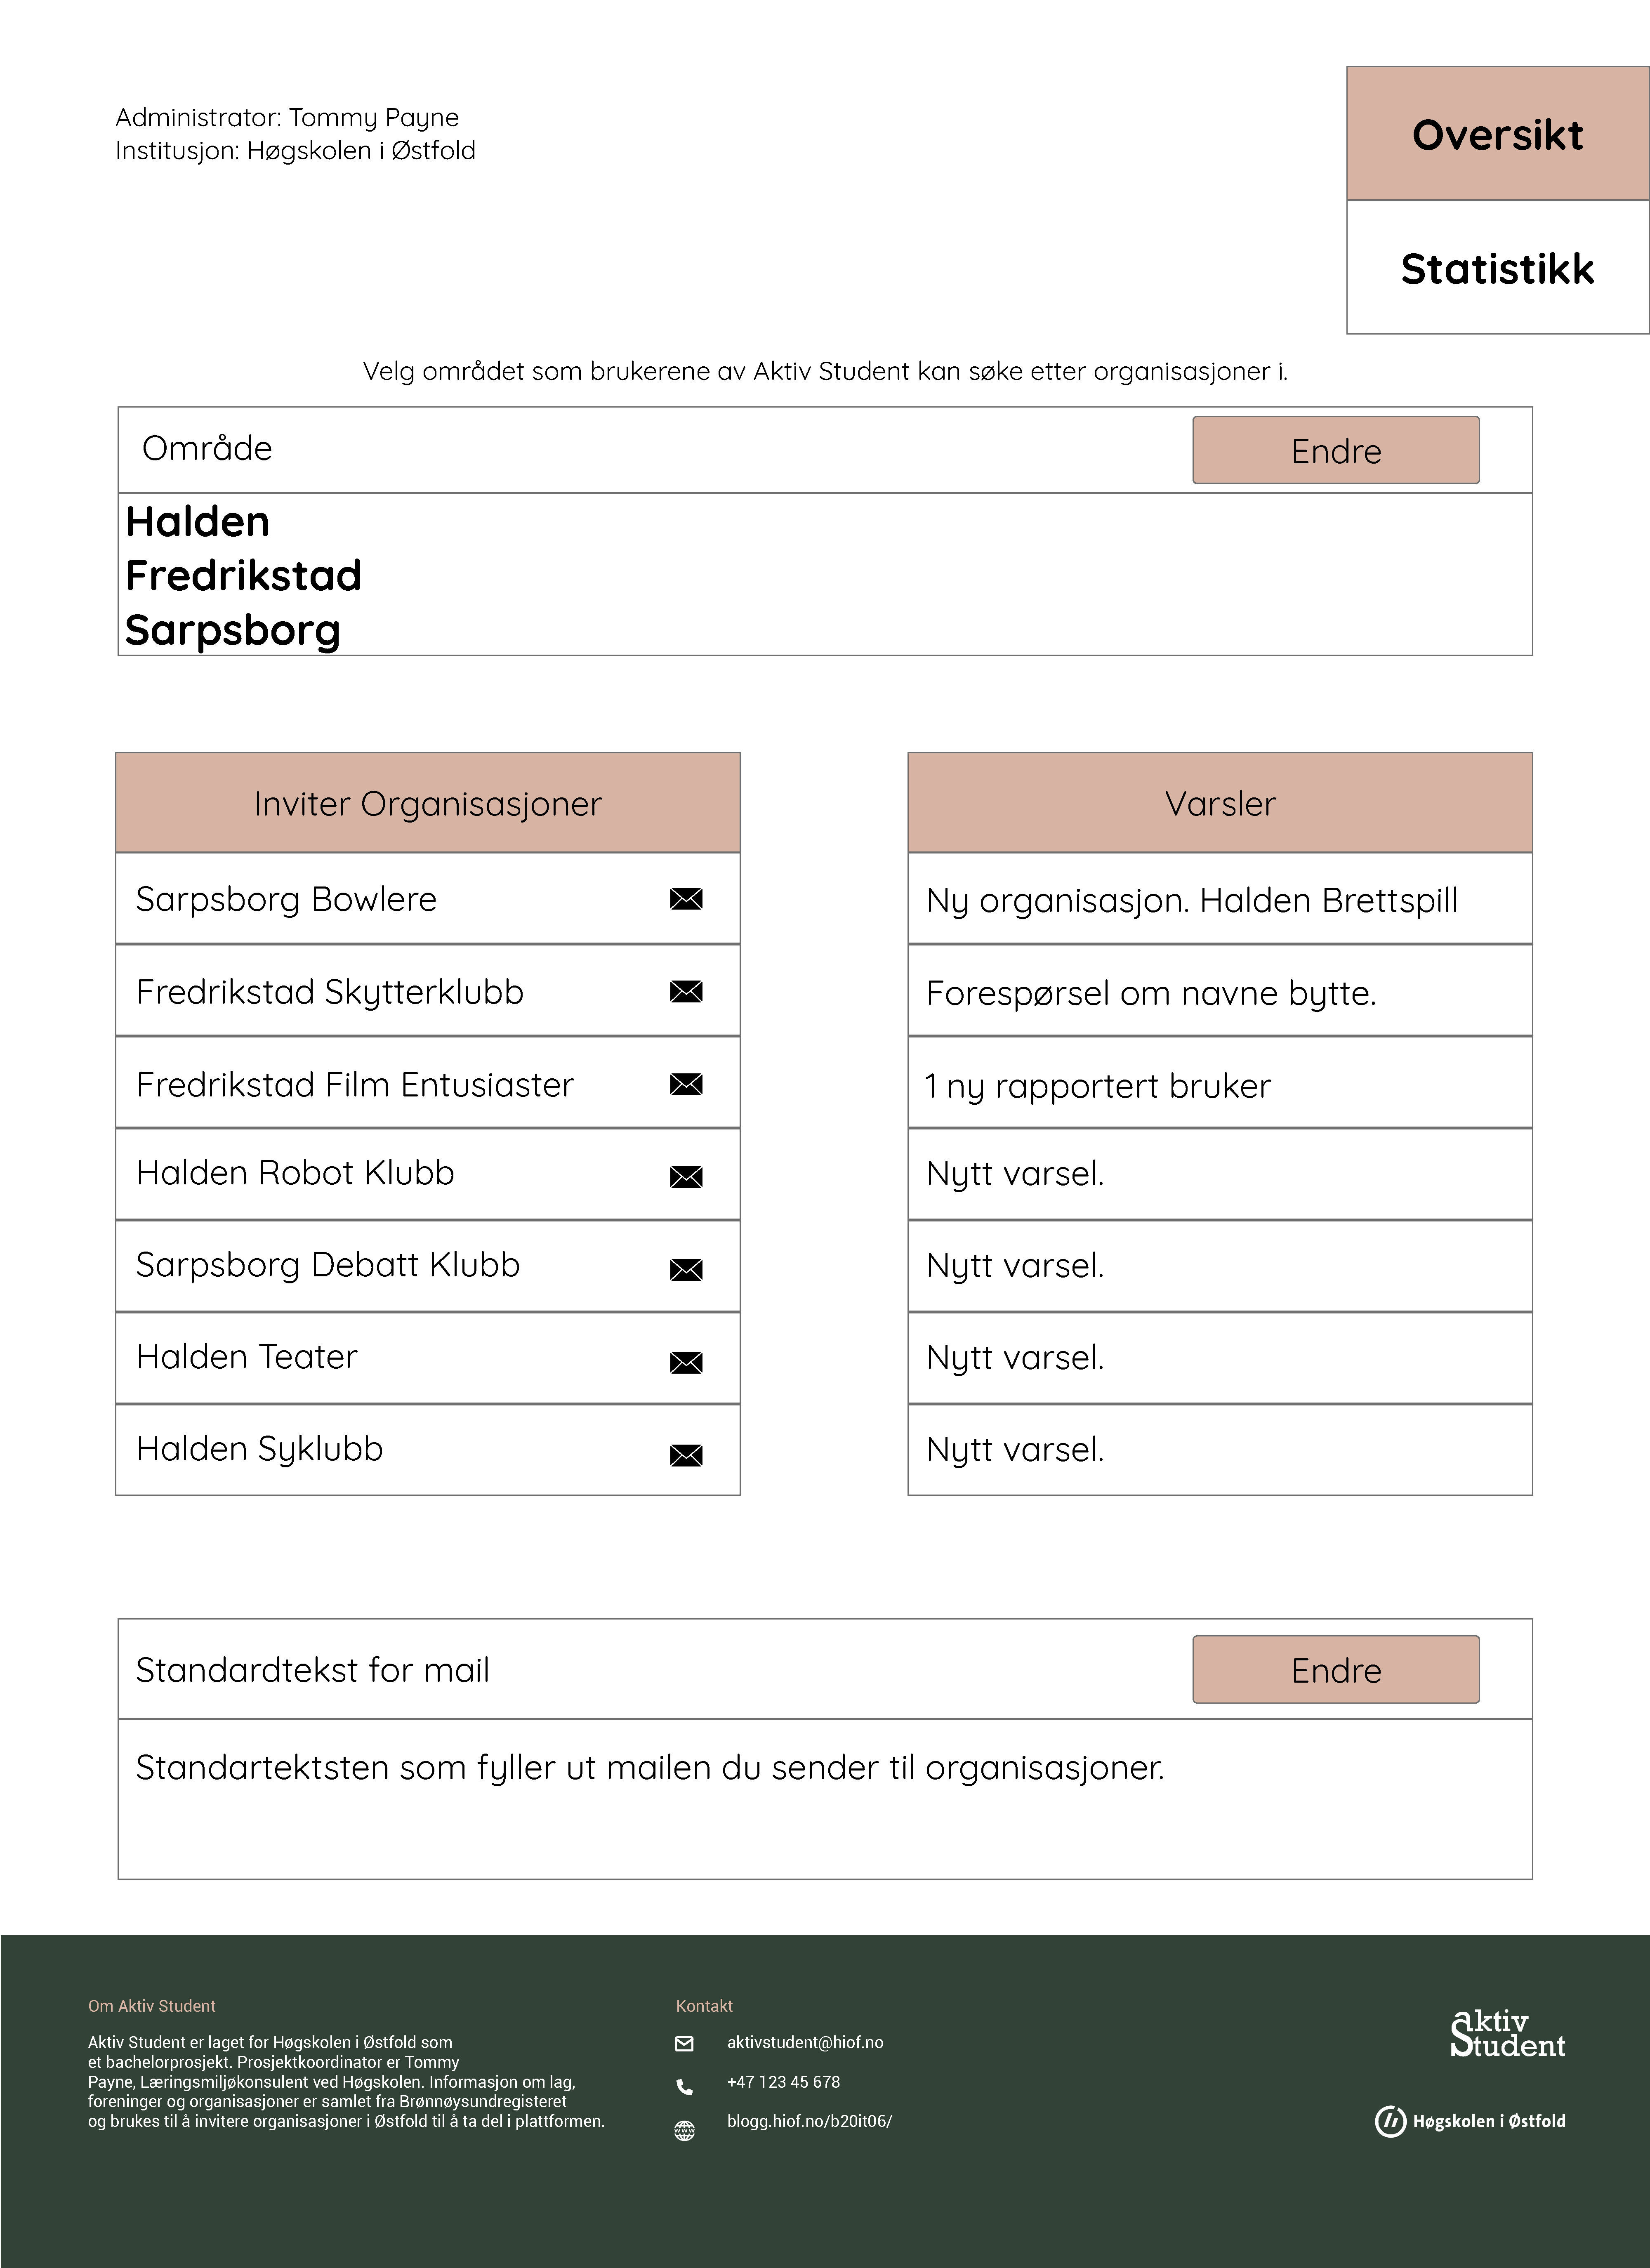
\includegraphics[width=.9\textwidth]{Illustrasjoner/Skisser-pdf/3.0/3-19-admin-oversikt.pdf}
\caption{Adobe XD-skisse av hvordan administrator ser oversiktsdelen av administratorpanelet}
\label{vedlegg:3-19-admin-oversikt}
\end{figure}

\section{Administratorpanel statistikk}

\begin{figure}[H]
\centering
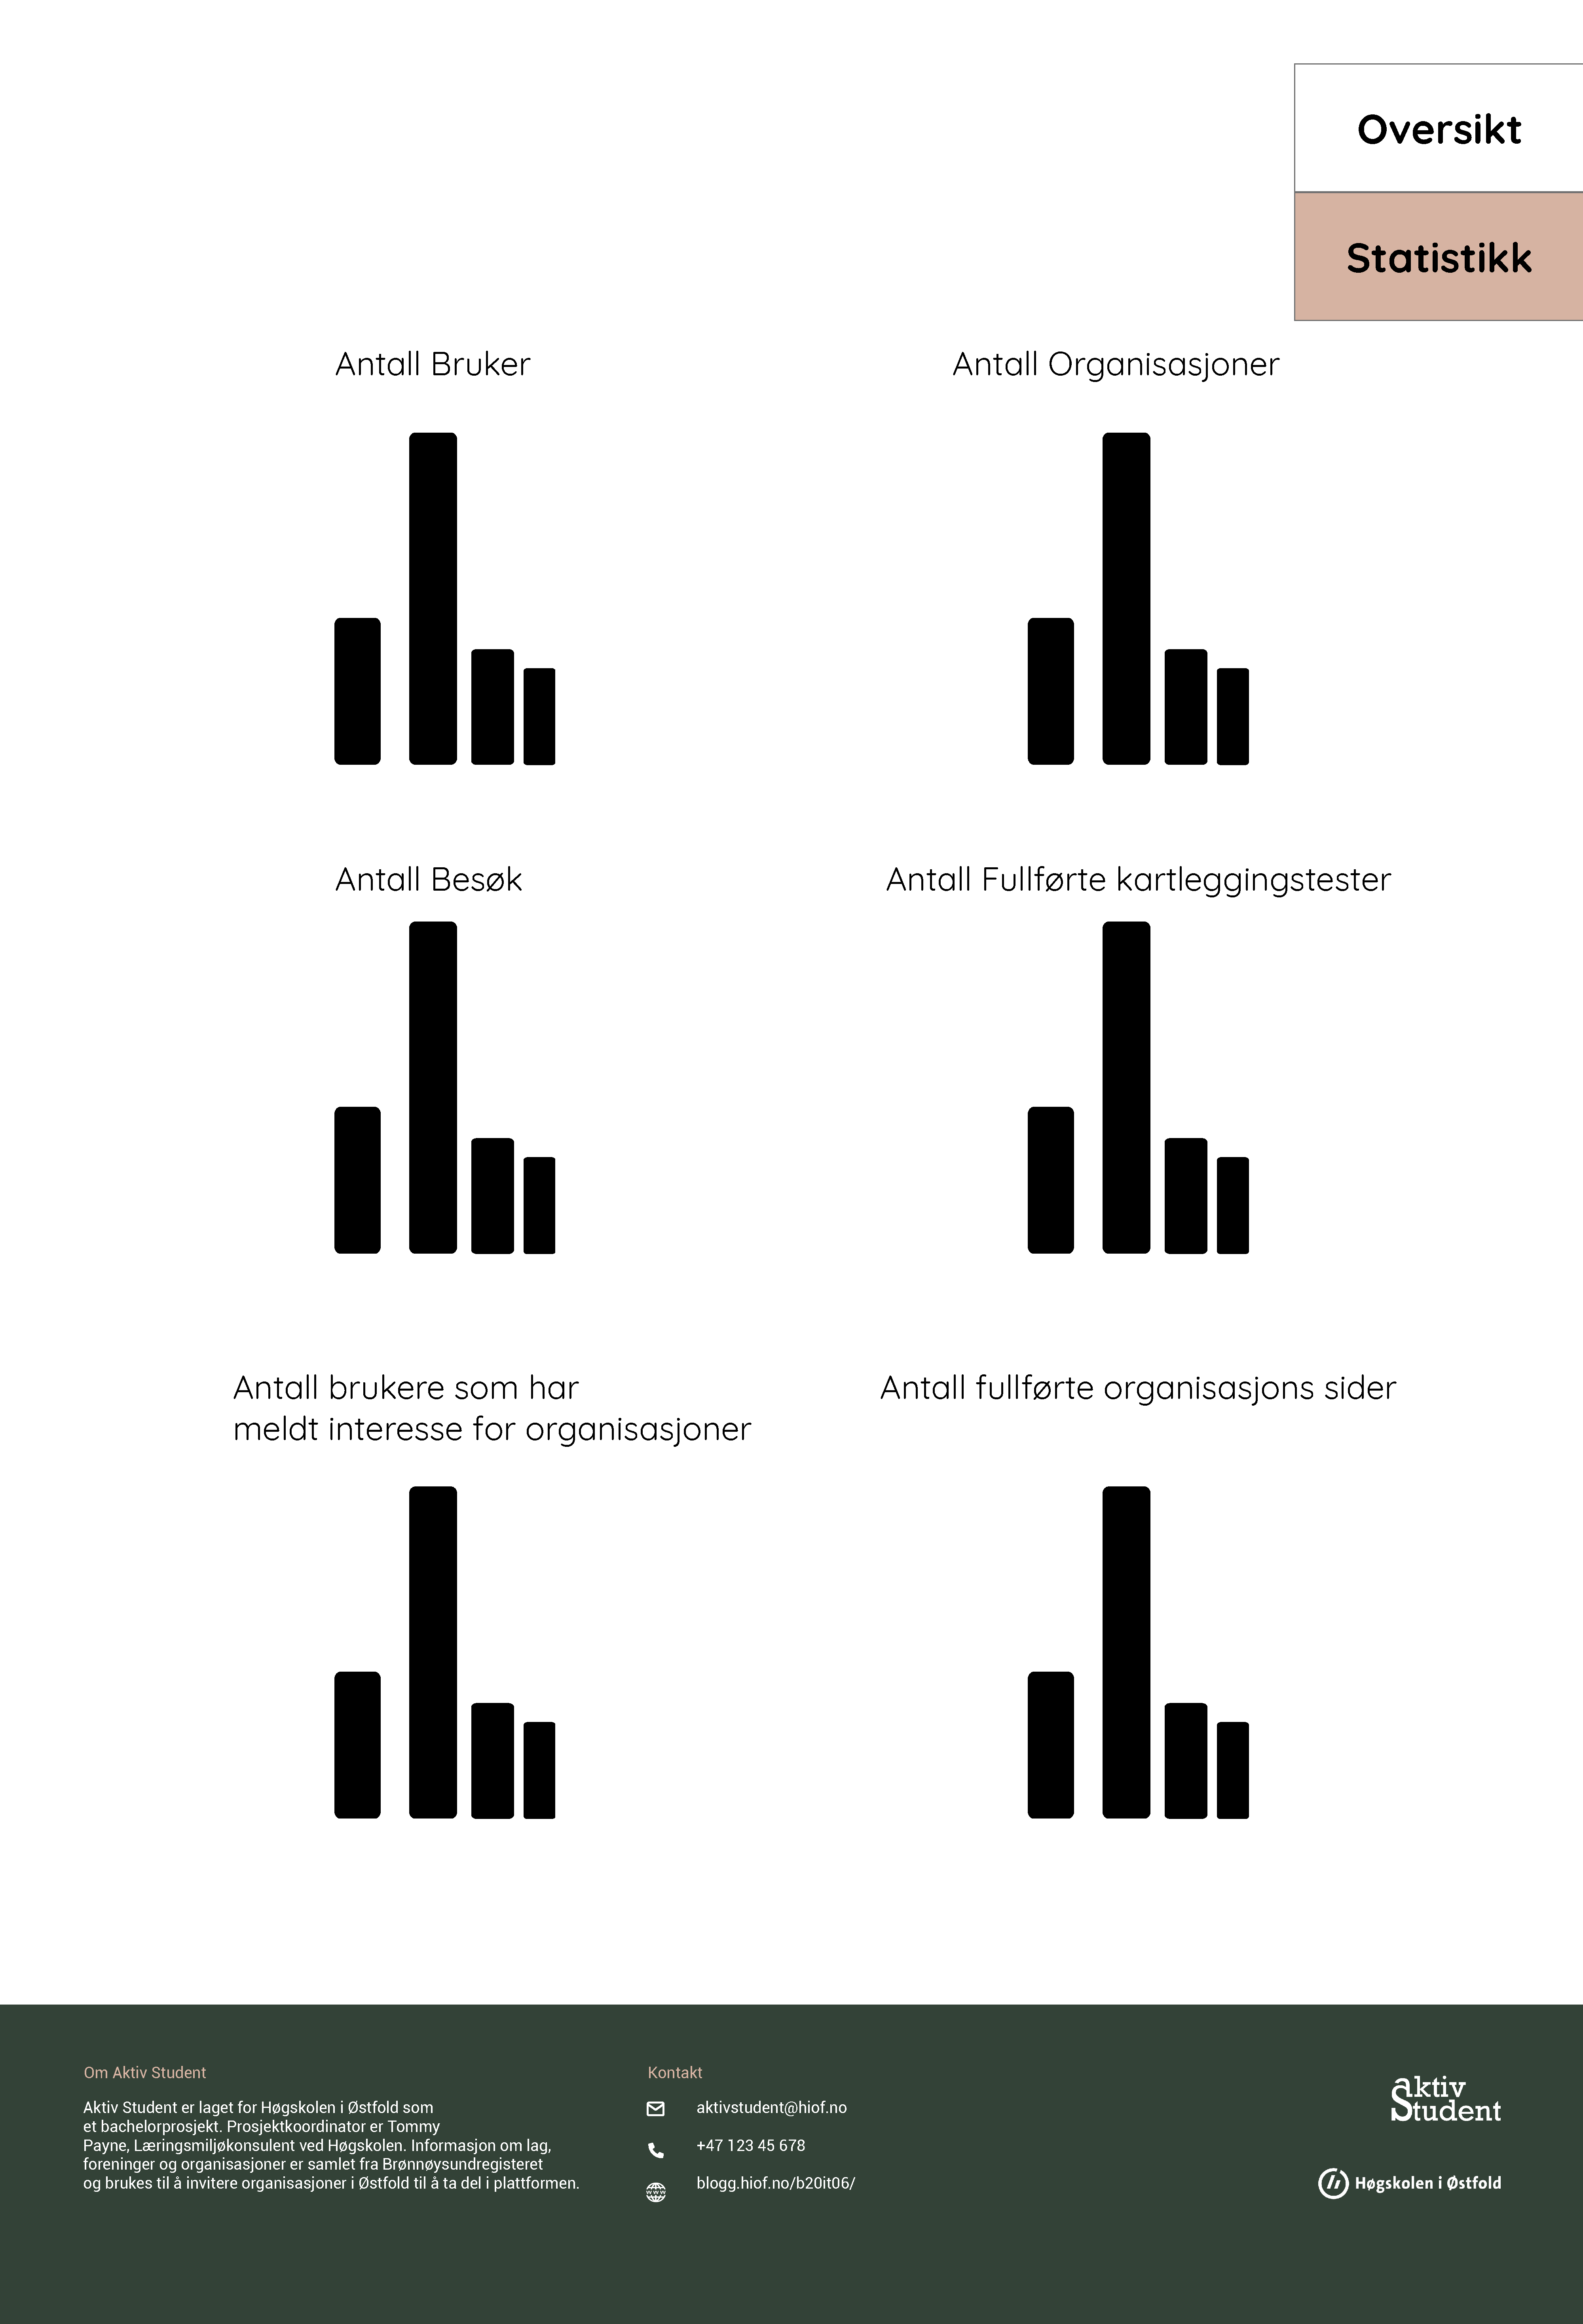
\includegraphics[width=.9\textwidth]{Illustrasjoner/Skisser-pdf/3.0/3-20-admin-statistikk.pdf}
\caption{Adobe XD-skisse av hvordan administrator ser statistikkdelen av administratorpanelet}
\label{vedlegg:3-20-admin-stats}
\end{figure}


